% ============================================================================
%  Elsevier submission front-end.
%
%  Same sections/ as main.tex -- only the class, the front matter and the
%  Elsevier-mandated sections differ. Edit the section files, never this
%  preamble's duplicate of them (there is none, by design).
%
%  TARGET JOURNALS (both Elsevier, both take elsarticle):
%    1. Environmental Modelling & Software  -- primary. Requires the
%       "Software availability" block below; it is not optional there.
%    2. Ecological Informatics              -- fallback, same class.
%
%  BUILD:  latexmk -pdf main-elsevier.tex
%  Overleaf: upload this file, sections/, tables/, figures/, refs.bib.
% ============================================================================

\documentclass[preprint,review,12pt,authoryear]{elsarticle}

% utf8 is the default on current TeX Live and a no-op there, but an
% Overleaf project pinned to an older compiler needs it, and the author
% names contain Turkish characters.
\usepackage[utf8]{inputenc}
\usepackage[T1]{fontenc}
\usepackage{textcomp}
\usepackage{lmodern}
\usepackage{microtype}
\usepackage{graphicx}
\graphicspath{{figures/}}
\usepackage{booktabs}
\usepackage{longtable}
\usepackage{amsmath,amssymb}
\usepackage{siunitx}
\usepackage{xcolor}
\usepackage[hidelinks]{hyperref}

% group-separator: the figures print 742,591 and the text must agree.
% group-minimum-digits stays at 5 (the default) on purpose -- at 4 the years
% written as \num{2015} would print as 2,015.
\sisetup{detect-weight=true, per-mode=symbol,
         group-separator={,}, group-minimum-digits=5}

% Long camelCase identifiers set in \texttt{} cannot be hyphenated, so a
% paragraph holding one (observedPropertyDeterminandCode, AssessedObservation)
% overflowed the measure by nearly 30 mm -- text protruding into the margin.
% \emergencystretch alone leaves three such boxes; hyphenat's htt option
% clears all of them. It costs ~30 "Font shape ... undefined" notices in the
% log, because Latin Modern has no bold small-caps typewriter for hyphenat to
% ask after; pdflatex substitutes a valid shape and the printed page is
% unaffected. A log notice is cheaper than a line in the margin.
\emergencystretch=3em
\usepackage[htt]{hyphenat}

% Unresolved values. Deliberately loud; none may survive to submission.
\newcommand{\pending}[1]{\textcolor{red}{\textbf{[TO COMPUTE: #1]}}}
% Values that came from a script; the argument is the file that produced them.
\newcommand{\src}[1]{\,\footnote{Produced by \texttt{#1}.}}

% elsarticle provides NO `highlights` environment, and an undefined
% environment inside frontmatter takes the whole frontmatter down with it --
% which is why the abstract was not appearing at all. Elsevier wants highlights
% as a separate upload; defining it here keeps the manuscript self-contained
% and visible to the editor.
\newenvironment{highlights}
  {\section*{Highlights}\begin{itemize}\setlength{\itemsep}{0pt}}
  {\end{itemize}}

\journal{Environmental Modelling \& Software}

\begin{document}

\begin{frontmatter}

% "detection limits" -> "reporting limits": WISE-6 has no detection-limit
% field, both provisions at issue are written about the quantification limit,
% and "reporting limit" is the umbrella term the censored-data literature this
% paper builds on uses (Helsel; Section 2.1). The ontology models both limits,
% so the old title was not false -- but it promised a quantity the data do not
% carry, which is the first thing a referee checks.
% Shortened after the colon, not before it. "compliance that cannot be
% determined" was a five-word relative clause doing the work of one adjective,
% and "undecidable" is the word the paper already uses for the quantity it
% reports (43.8 % undecidable as reported), so the title now matches the
% vocabulary of the results. Every element is kept: reporting limits (chosen
% over "detection limits" for the reason below), the third outcome, and the
% domain -- an EM&S reader needs "micropollutant monitoring" to place the work.
% A shorter variant, if 115 characters is still too many, ends at
% "...undecidable compliance in water monitoring" (107).
\title{Not detected is not absent: an ontology for reporting limits
and undecidable compliance in micropollutant monitoring}

\author[bu]{Recep Can Altınbağ\corref{cor1}}
\ead{recep.altinbag@bogazici.edu.tr}
\author[itu]{Mehmet Tahir Sandıkkaya}
\author[bu]{Ulaş Pekyavaş}
\cortext[cor1]{Corresponding author.}
\address[bu]{Institute of Environmental Sciences, Boğaziçi University,
TR34342 Beşiktaş, Istanbul, Türkiye}
\address[itu]{Department of Computer Engineering, Istanbul Technical
University, TR34469 Sarıyer, Istanbul, Türkiye}

\begin{abstract}
Micropollutant records are full of \emph{non-detections}: the analyte was
sought and not found, so the result is a bound, not a value, yet stored as a
number. Article~3(3b) of Directive 2008/105/EC excludes such a result from
status assessment where its limit exceeds the standard, which a two-valued
record cannot express.

Auditing the European Environment Agency's Waterbase (\num{4190833} river
station-years, \num{637} substances, \num{37} countries) finds \num{44.9}\% of
samples below the quantification limit and \num{40.1}\% of assessments from a
method failing Directive 2009/90/EC. The two failures have different histories:
station-years declaring neither a censoring flag nor a limit --- \num{25.5}\%
overall --- are absent after \num{2012}, when the set of reporters also changes,
whereas since \num{2020} \num{19.3}\% of assessments are still below-quantification
results whose limit exceeds the standard, so the analytical failure is not an
artefact of an archive. Substitution manufactures findings: the same records yield
\num{59251} to \num{200708} exceedances as non-detections enter at zero, half
the limit or the limit, \num{112034} created by the substitution alone and only
\num{14809} affirmable in law. The \num{2026} standards are applied to a record that
predates them: the test is what the monitoring can decide, not who breached
what.

CENSO is an OWL~2 ontology on SOSA/SSN whose central choices the record decides.
The quantification limit is not a property of the instrument: \num{56.4}\% of
multi-year station--substance pairs carry more than one, which a threshold column
cannot hold, and CENSO carries the bound each limit implies onto the result it
qualifies. Compliance is three-valued --- met, not met, or not determinable, the
outcomes the Directive admits --- the third subtyped by the reason, which keeps
an unmeasurable standard apart from an unreported bound. Of \num{696168}
station-years a European standard reaches, \num{38.4}\% are undecidable, and the
largest single reason is analytical: \num{18.2}\% are below-quantification results
Article~3(3b) sets aside. The other half arises before any limit meets any
standard --- \num{19.2} points with no bound at all or with a standard written
over a quantity the record does not supply, once the water hardness the release
reports on rows of its own is joined and the first tier of the EU bioavailability
guidance is applied; read row by row, without that join, \num{43.8}\% are
undecidable. Swapping the regulation package re-decides
\num{16.0}\% of co-regulated outcomes. Of \num{21} ontologies parsed --- reaching outside the water domain to
the analytical-chemistry vocabularies, one of which defines the quantification
limit from the IUPAC Gold Book and still binds it to the method --- none carries
a censoring status, and \num{20} cannot separate a non-detection from a
measurement at the same number. In CENSO that distinction is an inconsistency,
not a label. Ontology, pipeline and figure data are open.

\end{abstract}

\begin{keyword}
limit of quantification \sep censored data \sep environmental quality standards \sep
micropollutants \sep compliance assessment \sep Water Framework Directive \sep
ontology \sep open world assumption
\end{keyword}

\end{frontmatter}

%% Elsevier highlights: 3--5 bullets, each at most 85 characters.
\begin{highlights}
% Every numeral here is inside \num{} so that scripts/99_audit.py sees it.
% These bullets carried 47 %, 908 of 10,065 and 18.5 % long after the threshold
% table was corrected, because plain digits are invisible to the claim checker
% -- and the highlights are the first thing a reader of the article page sees.
% "EU assessments" was the overclaim a referee reaches for first: these are OUR
% assessments of a reported record against the standards in force in 2026, not
% assessments the reporting authorities performed, and only 8 of the 37
% reporters have a post-2015 river record (Section 5.2). "Under standards now in
% force" carries the counterfactual; "assessable station-years" carries the
% denominator. Six bullets also broke Elsevier's 3--5 rule; the precondition
% bullet is parked below and can be swapped for any of these five.
\item EU law mandates a third outcome that no surveyed vocabulary can express
\item Under standards now in force, \num{40.1}\% of assessable station-years fail the LOQ test
\item \num{25.5}\% of river station-years record neither a censoring flag nor a limit
\item Substitution invents \num{112034} of the \num{171285} exceedances it reports
\item Swapping the regulation package changes \num{17.7}\% of co-regulated verdicts
% \item \num{18.8}\% of assessable station-years meet a standard's precondition nowhere
\end{highlights}


%% ---------------------------------------------------------------------------
%% Software availability --- required by Environmental Modelling & Software.
%% ---------------------------------------------------------------------------
\section*{Software availability}
\noindent
\begin{tabular}{@{}p{0.28\linewidth}p{0.66\linewidth}@{}}
\textbf{Name} & CENSO (ontology) and the accompanying analysis pipeline \\
\textbf{Developer} & Recep Can Altınbağ, Boğaziçi University \\
\textbf{Contact} & recep.altinbag@bogazici.edu.tr \\
\textbf{Year first available} & 2026 \\
\textbf{Hardware required} & Any; the full pipeline runs on a laptop \\
\textbf{Software required} & Python 3.8 or later. No JVM and no external
  reasoner: OWL~2~RL entailment via \texttt{owlrl}, closed-world validation via
  \texttt{pyshacl}. Dependencies pinned in \texttt{requirements.txt} \\
\textbf{Program language} & Python; ontology in OWL~2 (Turtle and RDF/XML);
  constraints in SHACL; queries in SPARQL \\
\textbf{Program size} & Ontology \textasciitilde{}60~kB across three modules
  plus two regulation packages; pipeline \textasciitilde{}250~kB \\
\textbf{Availability and cost} & Free and open. Ontology and regulation
  packages under CC~BY~4.0 at \url{https://w3id.org/censo/}; code under MIT.
  Archived at \pending{Zenodo DOI} \\
\end{tabular}

\vspace{1em}
\noindent
Every number reported in this paper is produced by a script and written to a
file under \texttt{eval/}; none is typed by hand. \texttt{scripts/99\_audit.py}
recomputes each claim from the source data rather than checking that the value
appears somewhere, and fails if any claim cannot be reproduced.

\section{Introduction}

Trace organic contaminants -- pharmaceuticals, pesticides, biocides, UV filters
-- are ubiquitous in surface
waters~\cite{schwarzenbach2006challenge,loos2009eu}. A global river survey found
pharmaceutical contamination on every continent, exceeding safe concentrations
at a quarter of the sites~\cite{wilkinson2022pharma}. Pesticide concentrations
European regulation treats as acceptable are associated with losses of regional
stream invertebrate biodiversity~\cite{beketov2013biodiversity}; the substances
outpace the frameworks built to manage them~\cite{geissen2015emerging}.

These substances are regulated in the European Union through environmental
quality standards (EQS) under the Water Framework Directive~\cite{eu2000wfd},
transposed in T\"urkiye as \emph{\c{C}evresel Kalite Standartlar{\i}} (\c{C}KS).
Compliance is assessed by comparing measured concentrations against those
standards, a comparison less well defined than it appears.

Most such measurements are non-detections. The analyte is sought and not found.
That establishes an \emph{upper bound}, not absence: the substance may be
present below the method's limit of detection (LOD). The statement is
open-world.

Reporting practice replaces that statement with a number, usually zero or half
the limit of quantification (LOQ). Helsel showed that substitution fabricates
data and distorts every derived statistic~\cite{helsel2006fabricating}; the
point is not contested. It remains standard because \textbf{the data models in
use cannot hold the statement}. A relational table is closed-world: an absent
assertion is false, and a column of concentrations has no cell for ``present or
absent, below \num{0.02}\,\si{\micro\gram\per\litre}''. Substituting a zero is
not a rounding convention but a type error: it destroys the modality of the
measurement, not its magnitude.

Regulatory assessment implicitly requires three verdicts -- compliant,
exceeding, and \emph{cannot be determined}. The systems producing it can express
only the first two. Where the LOQ lies above the EQS, a laboratory can correctly
report ``not detected'' for a sample that may exceed the legal limit by two
orders of magnitude, and a closed-world pipeline records it as compliance.

Article~3(3b) of the consolidated Directive requires that a below-quantification
result whose limit exceeds the standard ``shall not be considered'' for status
assessment, and Article~4(1) of Directive 2009/90/EC requires that limit to sit
at or below \num{30}\,\% of the standard. Both mandate an outcome a two-valued
data model cannot represent, so neither can be audited from the data as
recorded.

We measure the cost in the European Environment Agency's Waterbase, the
monitoring Member States report under the Directive~\cite{eea_waterbase}:
\num{4190833} river station-years over \num{637} substances. Waterbase records a
below-quantification flag and the limit in force for each station, substance and
year, so where these are missing that absence is itself the measurement. We
quantify the share of samples below the quantification limit, the share of
station-years carrying neither flag nor limit, and the share assessed with a
method failing the legal performance criterion. Splitting the record at
\num{2015} separates a record-keeping failure the reporting authorities have
since repaired from an analytical one they have not; reading the disaggregated
release extends the audit to the standard Annex~I defines against a single
sample rather than against an annual mean.

The gap follows from a measurement model. SOSA/SSN and its descendants were
designed for in-situ \emph{sensing}, in which a detection limit is a property of
the device. Trace organic monitoring is \emph{sampling followed by laboratory
analysis}, in which the limit belongs to the method that produced the result
and its consequence belongs to the result itself. We present CENSO, an ontology
that carries the limit onto the result, records why a result is
an interval, treats a threshold as a conditional judgement with preconditions,
and makes compliance three-valued --- met, not met, or not determinable ---
subtyped by the reason it is not. The three are the outcomes the Directive
itself admits; the subtypes are what tell an unmeasurable standard apart from an
unreported bound. We also assess \num{21} ontologies, parsing each file rather
than reading its documentation, and the set reaches outside the water domain to
the analytical-chemistry and statistics vocabularies where these concepts would
live if they lived anywhere.

The ontology is the instrument, not the result. Without a vocabulary that
separates \emph{compliant} from \emph{cannot be determined}, none of the
quantities reported here can be counted at all.

\section{Related work}

\subsection{Censored environmental data}
Concentrations reported below a reporting limit are \emph{left-censored}.
Substituting a constant for them biases means, variances and trends by an
amount that depends on the censoring rate
\cite{helsel2006fabricating,helsel2012nondetects}, and Antweiler and Taylor
show it directly by treating coincident uncensored data as ground
truth~\cite{antweiler2008censored}. Robust alternatives -- regression on order
statistics, maximum likelihood estimation, Kaplan--Meier -- exist and go unused
in routine practice~\cite{shoari2018nondetects}. Our concern is upstream of all
of them: censoring status is discarded before the analyst opens the table, and
no estimator recovers what the schema could not hold.

\subsection{Observation vocabularies}
In SOSA/SSN \cite{janowicz2019sosa,haller2019ssn}, \texttt{sosa:Observation}
carries \texttt{hasSimpleResult}, a point value;
\texttt{ssn-system:DetectionLimit} is a property of a \emph{sensor}, never of an
observation or its result, so nothing can state that a measurement fell below
it. SOSA's \texttt{Sampling}, \texttt{Sampler} and \texttt{Sample} do not link
an analysis to a detection limit either, so the absence is not repaired by
choosing the sampling half of the vocabulary over the sensing half.
Section~\ref{sec:results-gap} shows why: the same absence appears in an
analytical chemistry ontology that has no sensor concept in it at all. What
these vocabularies share is not a model of measurement but a placement --- the
limit is held on whatever produced the result, and never on the result.

\paragraph{Why extend SOSA rather than something else.}
The choice of base is itself a claim, so we state the reasoning. SOSA/SSN is a
joint W3C Recommendation and OGC standard, which no alternative in this space
matches, and it is what the monitoring vocabularies compared in
Section~\ref{sec:results-gap} are built on --- so extending it is what makes the
diagnosis actionable for them rather than an argument for a parallel stack. We
add classes and properties and redefine no SOSA term. Three alternatives were
considered. \emph{O\&M / OMS} (ISO~19156), of which SOSA is the lightweight
\textsc{owl} rendering, does carry a \texttt{resultQuality} slot; but it is
typed to accept any data-quality element, so it is somewhere to put a string
rather than a modality a query can return, and the distinction between a bound
and a measurement is exactly what an unconstrained slot fails to preserve.
\emph{QUDT} and \emph{OM} model units and quantities, which CENSO reuses rather
than replaces. A \textsc{bfo}-grounded design in the \textsc{obo} style would
buy rigour at a cost that lands precisely on this subject matter: ``the record
cannot decide'' is an epistemic state of a document, not an entity in the world,
and representing absence and non-findings is a long-standing difficulty in that
tradition. The commitment we make instead is narrower and checkable --- the
vocabulary stays inside OWL~2~RL --- verified against the profile grammar
rather than assumed, which Section~\ref{sec:results-profile} reports --- and
what the profile cannot express is stated
and moved to SHACL rather than asserted and left unenforced.

\subsection{Water-quality exchange standards}
\label{sec:related-exchange}
Censoring is not unrepresented in water-quality data exchange, and the claim
this paper makes has to be stated against the standards that do carry it. OGC
WaterML~2.0~\cite{ogc2014waterml2} attaches a \texttt{censoredReason} to a
time--value pair and admits a censoring threshold as an untyped point-level
\texttt{qualifier}; ODM2~\cite{horsburgh2016odm2} and CUAHSI WaterML~1.1 carry a
censor code (less-than, non-detect, present but not quantified) on every value;
the SeaDataNet measurand qualifier flags~\cite{nerc_l20}, published as SKOS,
separate a value below detection from one below the limit of quantification;
and the US EPA Water Quality Exchange schema~\cite{epa_wqx3} goes furthest,
recording a detection condition and, on each result, any number of typed
detection and quantitation limits. \textbf{A censored result with its own limit
is therefore expressible today}, in XML and relational exchange formats
(Table~\ref{tab:exchange}). Three
things are not. In the SeaDataNet flags and in ODM2 the limit occupies the value
slot, so a reported number and the limit it was measured against cannot both be
kept. None of these standards is an ontology in which the limit, the result and
the applicable standard are related by axioms a reasoner or a shape can act on:
WQX can list a water-quality criterion among a result's limits, but as one more
limit type and not as a comparison. And none has a compliance outcome, so the
third outcome Article~3(3b) requires, and the reason it was reached, has nowhere
to go. The claim of this paper is confined accordingly. It is not that a
non-detection cannot be flagged; it is that no surveyed vocabulary or exchange
standard provides, in RDF/OWL, a result-level bound tied to the limit it came
from and to a three-valued verdict against a conditional standard.

\subsection{Laboratory and analytical vocabularies}
The concepts CENSO adds would most plausibly already exist not in a water
ontology but in a laboratory one, so the comparison in
Section~\ref{sec:results-gap} includes them. \textbf{CHMO, the \textsc{obo}
Chemical Methods Ontology, does declare \texttt{limit of detection} and
\texttt{limit of quantification}, both defined from the IUPAC Gold Book.} It
binds them to the method, as a \texttt{figure of merit} of an assay, and has no
property relating a limit to a result --- so, as with the sensor case, the limit
is known about the procedure and forgotten about the measurement. AFO, built by
a pharmaceutical consortium for analytical instrument data, contains no
detection or quantification limit term at all; its \texttt{lower bound} and
\texttt{upper bound} are \textsc{bfo} roles rather than values on a result. In
STATO, where censoring is a routine concept in survival analysis, it appears
only in prose. The gap is therefore not an artefact of having looked only at
water: the vocabulary that defines the limit most carefully still cannot say
that a given result fell below one.

\subsection{Water domain ontologies}
Water-quality vocabularies are plentiful~\cite{water_onto_review}: WaWO+ for
river basins~\cite{olivafelipe2017wawoplus}, OPO~\cite{wang2020opo},
InWaterSense~\cite{jajaga2015expert,ahmedi2013wqm},
SAREF4WATR~\cite{etsi2025saref4watr}, the Water Health Open Knowledge Graph
(WHOW)~\cite{whow2023onto,whokg2025}, query technologies over
SSN~\cite{calbimonte2012ssw} and water-treatment
interoperability~\cite{saka2026acquirium}.

Treating a regulation as machine-readable rules rather than as numbers in a
column is not new outside this domain: compliance checking over building codes
has been built on the same idea~\cite{bouzidi2012compliance}. What that
literature does not face is a measurement whose result is a bound, so the
verdict it computes is always determinate.

WHOW is the closest prior work and, unlike most, publishes at a dereferenceable
IRI. Its \texttt{Range} class bounds an \texttt{ObservationValue}, reading
\texttt{<10} as $[0,10]$. \textbf{WHOW therefore does represent a censored
result as an interval}: this work extends it rather than filling a void. What it
does not record is why the interval exists: it does not separate censoring from
spread, does not tie the interval to its limit, and cannot pose an indeterminate
compliance outcome. Section~\ref{sec:results-gap} compares \num{21} ontologies;
none carries the epistemic status of the measurement, and
Section~\ref{sec:results-separation} shows what follows --- on one real record,
\num{20} of the \num{21} cannot tell a non-detection from a measurement
reporting the same number.

\paragraph{Analytical coverage already changes conclusions.}
Moschet et al.~\cite{moschet2014screening} find that the pesticides a routine
programme omits dominate the risk picture; Malaj et
al.~\cite{malaj2014continental} read continental-scale risk to freshwater
ecosystems from the Waterbase records of Section~\ref{sec:results-waterbase};
Kase et al.~\cite{kase2018estrogens} report estrogen standards below what
routine laboratories can quantify at all. They ask what better chemistry would
reveal; we ask what the record establishes as it stands. The answer is often
nothing, and no substitution rule repairs it. Ahkola et
al.~\cite{ahkola2024uncertainty} treat uncertainty as a quantity to estimate and
propagate; where the threshold falls inside $[0,\mathrm{LOD}]$ the measurement
did not discriminate, so no distribution can be placed over the verdict -- a
representational gap, not an estimation problem.

\paragraph{A fourth reason the Directive misses risk.}
Weisner et al.~\cite{weisner2022threereasons} give three reasons the Water
Framework Directive fails to identify pesticide risk: an outdated analyte list,
biased sampling sites, and thresholds outside the Directive going unconsidered.
Each concerns \emph{which} substances are looked for and \emph{where}; ours
applies to the listed substances at monitored sites, where the record often
cannot decide the question it was collected to answer. Coquery et
al.~\cite{coquery2005analytical} raised uncertain analytical capability when the
priority substance list was first implemented; the Commission's Watch List
review restates it~\cite{loos2024watchlist}. What is missing is a way to
\emph{count} the consequence, which requires representing the failure rather
than substituting past it.

\section{Data and regulatory sources}
\label{sec:materials}

\subsection{EEA Waterbase}
The measurements are the European Environment Agency's Waterbase --- Water
Quality ICM, aggregated release: surface-water monitoring reported under the
Water Framework Directive~\cite{eea_waterbase,eu2000wfd}. One row is one
station, substance and year, with the annual mean, its sample count, a
below-quantification flag and \texttt{procedureLOQValue}, the limit in force.
Where the last two are missing, the absence is itself the observation.
Coordinates come from the companion \texttt{SpatialObjects} release.

The release read is \texttt{v2025\_1}, table
\texttt{Waterbase\_v2025\_1\_T\_WISE6\_AggregatedData.csv}, downloaded on
\num{8}~July~\num{2026}: \num{6450192} rows. The version matters because the
EEA replaces a release in place at the same address, so the citation records the
archive's SHA-256 as well --- an address identifies where the file was, a digest
identifies which file it was.

River water only is retained: an inland-surface-water standard does not apply to
lakes, transitional or coastal waters. That leaves \num{4190833} station-years
over \num{4170005} distinct station--substance--year keys, a few being reported
as two rows where the year is split into sampling periods.

\textbf{Both rows are assessed, and the unit of every count in this paper is
therefore the published row rather than the station-year.} Of the
\num{696168} rows a European annual-average standard reaches,
\num{689266} carry a distinct station--substance--year and \num{6902}
--- \num{0.99}\,\% --- are a second or later row for a key already
seen\src{scripts/22\_waterbase\_external.py}. They are neither merged nor
dropped, for the reason that governs the rest of this work: each row is a
\emph{published} annual mean with its own \texttt{procedureLOQValue} and its
own below-quantification flag, the two may have been produced by different
methods with different limits, and the release states no rule for combining
them. Choosing one would be inventing the datum the record withholds. What the
choice can cost is bounded without making it: removing every duplicate row
moves the undecidable share of Section~\ref{sec:results-wbabox} from
\num{43.8}\,\% to between \num{43.2} and \num{44.2}\,\% --- at most
\num{0.56} percentage points --- whichever of the two rows a deduplicating
rule were to keep. The aggregated
release is used because an annual-average standard is defined against an annual
mean, which is what one row holds.

Only Annex~I's maximum allowable concentration, defined against a single
measurement, needs the disaggregated release of the same version
(\texttt{Waterbase\_v2025\_1\_T\_WISE6\_DisaggregatedData.csv}); the
aggregated file has averaged that quantity away and cannot evaluate it at any
level of effort (Section~\ref{sec:results-mac}). That release holds
\num{96597294} rows, of which \num{55358021} are river samples and
\num{8148785} carry a substance for which Annex~I states a maximum allowable
concentration.

\textbf{It is the less complete of the two, and the shortfall is reported
rather than assumed away.} Sample-level reporting is not uniform between Member
States: the disaggregated release reaches \num{1234302} of the
\num{4170005} river station-years, \num{29.6}\,\%, with a median of
\num{6} samples behind a covered station-year and quartiles of \num{4}
and \num{12}\src{scripts/27b\_disaggregated\_coverage.py}. The median is
quoted rather than the mean because the distribution is skewed: a few
station-years carry hundreds of samples and most carry a handful. Every
maximum-allowable result in Section~\ref{sec:results-mac} therefore describes
that covered stratum and is reported apart from the annual-mean results --- not
only as a coverage caveat, but because the two standards disagree on
\num{25.6}\,\% of the station-years readable both ways, and disagree in both
directions, so neither is a stricter version of the other. The SQLite distributions
duplicate the CSV releases and are unused; the by-water-body aggregation is a
different spatial unit, not comparable to a station-year.

\subsection{Regulatory thresholds}
Every threshold is transcribed from its primary text, never from a secondary
compilation.

\paragraph{Environmental quality standards.}
Annex~I of Directive 2008/105/EC, consolidated version in force on 10 May
2026~\cite{eu2008eqs,eu2013priority}, as amended by Directive~(EU)
2026/805~\cite{eu2026amend}. Parsing it is not
mechanical\src{scripts/10\_parse\_eu\_eqs.py}. Group standards apply to a sum,
not to any single substance, and are excluded from per-substance comparison.

\paragraph{The comparison is deliberately counterfactual.}
The standards in force in \num{2026} are applied to a record that predates them:
only \num{8} of the \num{37} reporting countries contribute station-years from
\num{2015} or later (Section~\ref{sec:results-era}). No reporter is in breach of
a rule that did not yet bind it, and nothing here should be read as such a
finding. The question is whether the monitoring, as performed and reported,
could decide the standards now in force --- a property of the data, not the
date. Where a number depends on the standard chosen,
Section~\ref{sec:results-dual} reports how far it moves under a different one.

\paragraph{Analytical performance.}
Article~4(1) of Directive 2009/90/EC requires ``a limit of quantification equal
or below a value of \num{30}\,\% of the relevant environmental quality
standards''~\cite{eu2009qaqc}, stricter than asking whether the limit exceeds
the standard outright. Section~\ref{sec:results-waterbase} reports both.

\paragraph{A second package, for swappability.}
Table~4 of the Turkish \emph{Yer\"ust\"u Su Kalitesi Y\"onetmeli\u{g}i} as
amended in \num{2016}~\cite{tr2012ysky} is transcribed the same
way\src{scripts/08\_verify\_thresholds.py} and released alongside, though not
analysed here, so that the swappability claim of
Section~\ref{sec:methods-packages} rests on two loadable jurisdictions, not on
an assurance.

\subsection{What is joined to what}
Substances are matched to thresholds by CAS registry number, carried in
\texttt{observedPropertyDeterminandCode}. Name matching was not used: names
diverge between a directive, a national register and a laboratory's sheet, and a
missed join would silently understate every count that follows. Concentrations
arrive in one column as \si{\milli\gram\per\litre}, \si{\micro\gram\per\litre}
and \si{\nano\gram\per\litre}; each is converted before comparison.
\section{Methods}
\label{sec:methods}

\subsection{CENSO: binding the limit to the result}
\label{sec:methods-vocab}
CENSO\footnote{\url{https://w3id.org/censo/}, CC~BY~4.0.} extends
SOSA/SSN~\cite{janowicz2019sosa,haller2019ssn} for observations from a method
with a detection limit, reusing PROV-O~\cite{w3c2013provo} for the analytical
run, SKOS~\cite{w3c2009skos} for substance concepts and QUDT for units;
substances are aligned to ChEBI~\cite{degtyarenko2008chebi} where an identifier
exists (\num{180} of \num{240}). It follows LOT~\cite{poveda2022lot} (successor
to NeOn~\cite{suarez2012neon}), whose competency questions produced the
evaluation in Section~\ref{sec:results-cq}, and is published for
reuse~\cite{wilkinson2016fair}. Four commitments distinguish it from the
vocabularies surveyed in Section~\ref{sec:results-gap}.

\paragraph{The limit is carried onto the result.}
\texttt{censo:AnalyticalMethod} is a \texttt{sosa:Procedure} carrying a unit and
at least one limit --- of quantification, of detection, or both, since a
constraint satisfiable only by inventing the missing datum constrains nothing.
That much CHMO also has, and puts in the same place
(Section~\ref{sec:results-gap}). The step that separates a bound from a
measurement is the next one: \texttt{censo:resultUpperBound} places the limit
on the \emph{observation}, so \emph{censored} is a property of a result and
not of the procedure that produced it. Two observations from one method, one
below the limit and one above, differ in exactly this.

An earlier version of the vocabulary reified the analytical run for the same
purpose. It is retired, for two reasons that are worth stating because the
commitment is unchanged. A run is a \texttt{prov:Activity} that used a sample
and generated an observation, and the method it executed already carries the
limits, so declaring our own terms for it reinvented \textsc{prov-o}. And no
European release reports a run identifier: an annual mean spans many runs, so
minting one per station-year would not simplify but misstate. Where a publisher
does have run-level provenance, \textsc{prov} expresses it with no extension,
and the bound it produces still lands on
\texttt{censo:resultUpperBound}.\src{scripts/99\_audit.py, \texttt{check\_no\_dead\_terms}}

\paragraph{The substances are reconciled, not renamed.}
A \texttt{censo:Analyte} is a \texttt{sosa:ObservableProperty} --- the
concentration \emph{of} a substance --- and not the substance, whose instances
are molecules. The two are related by \texttt{rdfs:seeAlso} to the substance's
ChEBI class, in a separate module the vocabulary does not
import\src{scripts/20\_align\_external.py}: \num{299} of \num{354} analytes
across the two packages resolve to exactly one ChEBI class by CAS registry
number, \num{26} resolve to more than one and are deliberately left unaligned,
and \num{29} --- technical mixtures and congener groups such as C10--13
chloroalkanes --- have no ChEBI entry at all, which is a fact about what the
regulation names rather than a gap in the mapping.

\texttt{owl:sameAs} is reserved for the relation that is an identity: two
packages' names for one observable property. \num{30} such pairs reconcile the
European and Turkish vocabularies, so the co-regulated stratum of
Section~\ref{sec:results-dual} is an entailment rather than a string join, and
the audit requires the two to agree --- every substance the analysis treats as
co-regulated must be reachable through a \texttt{sameAs} pair.

\paragraph{Detection status is explicit and exhaustive.}
\texttt{CensoredObservation}, \texttt{EstimatedObservation},
\texttt{QuantifiedObservation} and \texttt{UnresolvedObservation} are pairwise
disjoint and cover \texttt{AssessedObservation}. Never measured is a fifth
situation, carried by the absence of an observation rather than by a class:
under the open-world assumption that is how one says a measurement was not made.
It is the distinction a \texttt{WHERE concentration = 0} query cannot draw, and
conflating it manufactures findings.

\paragraph{A threshold is a conditional judgement.}
\texttt{censo:Threshold} carries a value, a unit, a citation to the regulation,
and \texttt{requiresCondition} links to \texttt{ApplicabilityCondition}
subclasses: matrix, analytical fraction, bioavailability basis, hardness class.
Where a precondition is unmet the outcome is \texttt{PreconditionUnmet}, one
of the four subclasses of \texttt{IndeterminateCompliance} --- not a default
pass. Annex~I
creates two such conditions in footnotes: the standards for lead and nickel
``refer to bioavailable concentrations of the substances'', and cadmium's
``vary depending on the hardness of the water as specified in five class
categories''. The released package attaches them, and
Section~\ref{sec:results-precondition} shows what they decide.

\paragraph{Compliance is three-valued, and the third value records why.}
\texttt{Exceedance}, \texttt{Compliant} and \texttt{IndeterminateCompliance} are
jointly exhaustive \emph{for a given observation--threshold pair}, and they are
what the Directive itself admits: the standard is met, it is not met, or
compliance cannot be determined. Why it cannot is carried by four subclasses of
the third --- \texttt{PreconditionUnmet}, \texttt{MethodInsufficient},
\texttt{PossibleExceedance} and \texttt{BoundNotEstablished} --- and not by a
fourth top-level value, which would be the vocabulary asserting a distinction
the Directive does not make. \texttt{PossibleExceedance} belongs there rather
than beside \texttt{Exceedance}: an interval straddling the limit decides
nothing, which is indeterminacy with a particular cause, and the assessment
reported in Section~\ref{sec:results-wbabox} has counted it that way throughout.

Where two subclasses describe one result --- a censored result whose limit
exceeds the standard has an interval straddling it too --- Article~3(3b) is
decisive and the observation is recorded under \texttt{MethodInsufficient}. That
precedence is a rule-layer priority and deliberately not an
\texttt{owl:disjointWith} axiom between the subclasses, for the same reason no
class-level disjointness is asserted among the three outcomes: a measurement may
legitimately be compliant under one jurisdiction's standard and indeterminate
under another's, and Section~\ref{sec:results-dual} depends on the graph holding
both. Exclusivity is carried instead by an \texttt{owl:AllDisjointProperties}
axiom over \texttt{exceeds}, \texttt{possiblyExceeds} and
\texttt{belowThreshold}, with the equivalent pairwise axioms alongside it
because the pure-Python engine used here implements only the pairwise rule.

Figure~\ref{fig:geometry} shows three real observations. Where the threshold
clears the censored interval (a), the non-detection decides the question and the
ontology returns \texttt{Compliant}: censoring is not an excuse for refusing
every verdict. Where it falls inside (b), no result the method could have
returned would have decided the question, and any substitution rule merely picks
one.

The panels are cut at the quantification limit: Waterbase reports
\texttt{procedureLOQValue} and no detection limit, and both provisions at issue
--- Article~3(3b) of Directive 2008/105/EC and Article~4(1) of Directive
2009/90/EC --- are written about that limit. Section~\ref{sec:methods-noise}
distinguishes a threshold below the detection limit from one between the two;
this source cannot show that on measured cases.

\begin{figure}[htbp]\centering
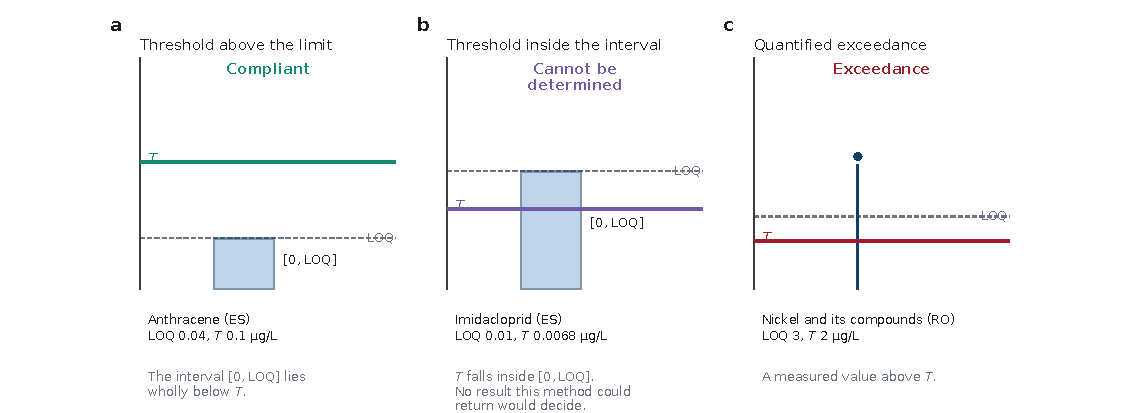
\includegraphics[width=\textwidth]{fig06_decision_geometry.pdf}
\caption{Why two verdicts are not enough, on three real observations. A
non-detection is the interval $[0,\mathrm{LOQ}]$ (shaded), not a value; the
threshold $T$ is a line. Panels (a) and (c) are decidable and a conventional
pipeline gets them right; panel (b) is not, and it is silently recorded as
compliant --- a distinction available to a reasoner but invisible to a numeric
column. Each panel is scaled to its own limit; substance, country and values are
in \texttt{supplementary/figure\_data/fig06\_decision\_geometry.csv}. Generated by
\texttt{scripts/90\_figures.py}.}
\label{fig:geometry}
\end{figure}

\subsection{Regulations as pluggable, versioned packages}
\label{sec:methods-packages}
Thresholds expire. \texttt{cereg:RegulationPackage} makes each regulation a
self-contained module of individuals with jurisdiction, dates and a
machine-readable \texttt{transcriptionStatus}, so unverified values can be
excluded rather than trusted. Two packages are released with the
ontology\src{scripts/19\_build\_regulation\_packages.py}: \texttt{tr-ysky-2016}
(\num{434} thresholds) and \texttt{eu-2008-105-2026} (\num{114} thresholds),
both transcribed from the primary legal texts and carrying
\texttt{VerifiedAgainstPrimarySource}. Each contributes individuals only --- no
class, no property --- so one loads safely alongside another; the validator
checks this. Their thresholds carry different IRIs, so the Turkish and European
assessments coexist in one graph instead of overwriting each other.

\subsection{Is this not simply what detection limits are for?}
\label{sec:methods-noise}
Limits of detection exist to separate signal from noise, and a laboratory
reporting ``not detected'' is doing the right thing; nothing here disputes the
analytical practice. Two statements are then conflated:

\begin{itemize}
  \item \emph{the measurement cannot resolve a value} -- true below the limit;
    and
  \item \emph{the concentration is zero} -- not established by the measurement.
\end{itemize}

The laboratory asserts the first, the database records the second. What is lost
is not a value but the \emph{bound}: a non-detection establishes $c \in
[0,\mathrm{LOD}]$, and \num{0.0} is a different claim, not a weaker one. The
method is chosen on analytical grounds, the threshold arrives later from a legal
instrument, and their relative position is accidental. Article~3(3b) of the
consolidated Directive 2008/105/EC provides that a result reported as less than
a limit of quantification that is itself above the EQS ``shall not be considered
for the purposes of assessing the overall chemical status of that water
body''~\cite{eu2008eqs,eu2009qaqc}. The law requires a third outcome and
requires it to be identifiable; a two-valued schema cannot represent it.
Section~\ref{sec:results-waterbase} reports how often it arises.

\subsection{Could a column have done this?}
\label{sec:methods-why}
A relational table with a \texttt{censored} flag and an \texttt{lod} column
yields every number in Section~\ref{sec:results-waterbase}; our analysis scripts
are plain Python over CSV, and we do not claim these quantities are otherwise
uncomputable. What the flag does not give:

\begin{enumerate}
  \item \textbf{Several regulations over one set of observations.} The Turkish
    and European assessments differ substantially
    (Section~\ref{sec:results-waterbase}); with packages that is a re-query,
    with a threshold column a re-implementation, and the two cannot be held at
    once.
  \item \textbf{Preconditions belong to the threshold, not the measurement.} A
    flag on the observation cannot express a condition on the standard.
  \item \textbf{Justification.} A defined class yields a derivation for each
    verdict; a boolean yields a value.
  \item \textbf{Transfer.} The pattern is domain-independent; a column in one
    team's spreadsheet is not.
\end{enumerate}

This paper demonstrates (1) and (2) on real data and (3) on the axiom suite;
(4) is design intent, evidenced only by the vocabulary's independence from the
water domain, and we mark it as such.

\subsection{What OWL does, and what it does not}
OWL supplies identity, taxonomy, disjointness, classification and explanation.
It cannot compare data values, so \texttt{exceeds}, \texttt{possiblyExceeds} and
\texttt{belowThreshold} are materialised by the rule layer, then classified. The
open-world assumption that makes CENSO right for censoring blocks inferring
``none of the above'', so \texttt{IndeterminateCompliance} is materialised under
a locally closed world in SHACL. We do not claim that a description-logic
reasoner computes compliance.

\subsection{What is counted, and what is inferred}
\label{sec:methods-inference}
Almost nothing here is an estimate. The shares in
Section~\ref{sec:results-waterbase} and the three-valued assessment in
Section~\ref{sec:results-wbabox} are counts over every river station-year in the
release, computed by arithmetic on four reported fields; there is no sampling
frame and no population parameter to estimate, so no interval is reported for
them. Two places depart from that and are treated accordingly. Where a quantity
is selected \emph{by} its own value --- the ranked substances of
Figure~\ref{fig:loqeqs}a --- the \num{95}\,\% Wilson interval is plotted,
because ranking puts the least certain estimates at the top. Where a proportion
is compared between groups, Section~\ref{sec:results-dual} reports the interval
for the comparison it rests on.

Two limits of that treatment are worth stating rather than leaving to a reader.
Station-years are clustered --- by station, substance, reporting country and year
--- so they are not independent observations, and no comparison here corrects for
that; the descriptive shares do not need it, and the group comparisons should be
read as differences between the populations counted rather than as tests. And the
denominator of the two legal criteria is itself a reported quantity: a
station-year with no limit cannot fail a test about limits, so every rate built
on them is a lower bound, and loosest where reporting is worst
(Figure~\ref{fig:country-practice}).

\subsection{Reproducibility}
\label{sec:methods-repro}
Every number in this paper is produced by a script and written under
\texttt{eval/}; none is typed by hand. The pipeline is deterministic and runs in
pure Python (\texttt{owlrl}, \texttt{pyshacl}), so no external reasoner is
required. The ontology was scanned with OOPS!~\cite{poveda2014oops};
FOOPS!\ \cite{garijo2021foops} is the FAIR assessment we report as not yet run
rather than assert. A generated manifest maps every numeric claim to its
artefact and script, and fails if one cannot be
traced\src{scripts/95\_numbers\_manifest.py}.

The vocabulary is scanned for modelling pitfalls with
OOPS!~\cite{poveda2014oops} and assessed for FAIR publication with
FOOPS!~\cite{garijo2021foops}. FOOPS!\ is run against the published IRI rather
than the local file, because content negotiation, version-IRI resolution and
registry presence are properties of the publication and not of a serialisation:
it returns \num{0.78}, passing \num{18} of \num{24}
checks\src{scripts/15\_foops.py}. The six that do not pass are of two kinds and
we separate them rather than report a score. Three are missing annotations --- a
citation, a publisher, an issue date --- properties of the file, repairable
without touching an axiom. Three are absence from a public registry, which no
edit to the file achieves. Neither kind bears on the modelling claims made here;
the full report is in \texttt{eval/foops\_assessment.md} and the cached service
response beside it, so the figure can be re-derived without a network.

\section{Results}

\subsection{How often the record cannot support its own verdict}
\label{sec:results-waterbase}
Waterbase records a below-quantification flag and the limit of quantification
in force for each station, substance and
year\src{scripts/22\_waterbase\_external.py}. Keeping river water only, since
an inland-surface-water standard does not apply to lakes or coastal waters,
leaves \num{4190833} station-years from \num{37} reporting countries.

\paragraph{Censoring is the normal case, not an edge case.}
\textbf{\num{44.9}\% of all samples lie below the limit of quantification.}
Figure~\ref{fig:europe-map} maps the stations: the pattern follows national
borders, not river basins.

\begin{figure}[htbp]\centering
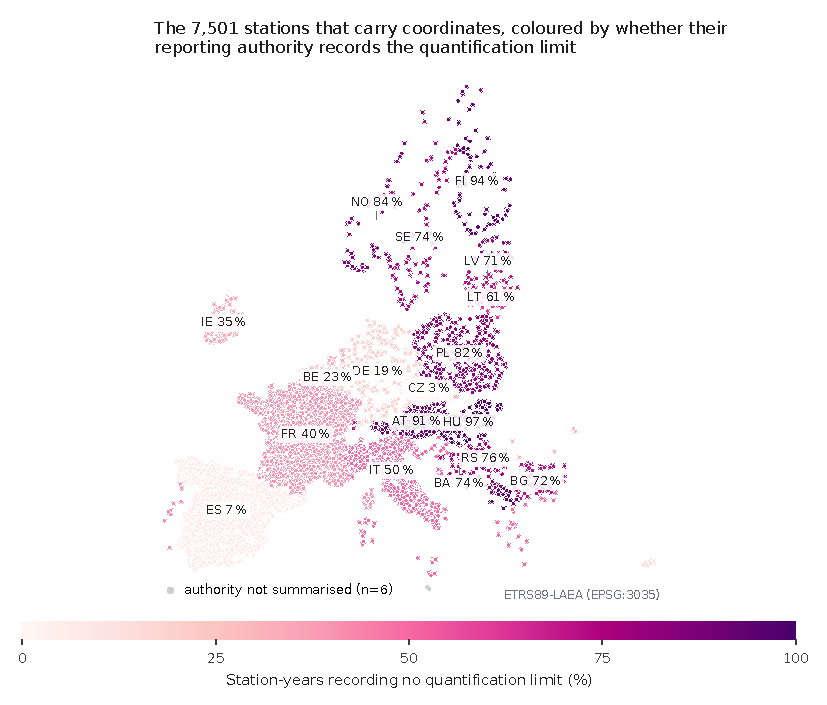
\includegraphics[width=0.86\textwidth]{fig02_europe_map.pdf}
\caption{The \num{7501} monitoring stations in the graph that carry
coordinates, in the equal-area projection the EEA publishes European water data
in (ETRS89-LAEA), coloured by the share of their reporting authority's
station-years that record no quantification limit. The value is a property of the
\emph{authority}, not of the station --- every station in a country carries the
same one --- so each national cluster is labelled with its code and its rate
rather than left to the colour scale alone. Countries are drawn lowest rate
first, so no reporter is hidden beneath another. No coastline is shown: no
boundary file is distributed with this work, and the outline of Europe here is
the monitoring network itself. The pattern follows national borders rather than
river basins, which places the defect in reporting practice rather than in
chemistry or hydrology. Every plotted station, with its country, is in
\texttt{supplementary/figure\_data/fig02\_europe\_map.csv}. Generated by
\texttt{scripts/90\_figures.py}.}
\label{fig:europe-map}
\end{figure}

\paragraph{The bound is missing for a quarter of the record.}
Where censoring is declared the limit is almost always recorded. The failure is
elsewhere: \textbf{\num{25.5}\,\% of station-years declare nothing at all}, no
flag and no limit, so a zero and a measured trace are indistinguishable and no
substitution rule can be chosen. These are \texttt{UnresolvedObservation} at
continental scale.

\begin{figure}[htbp]\centering
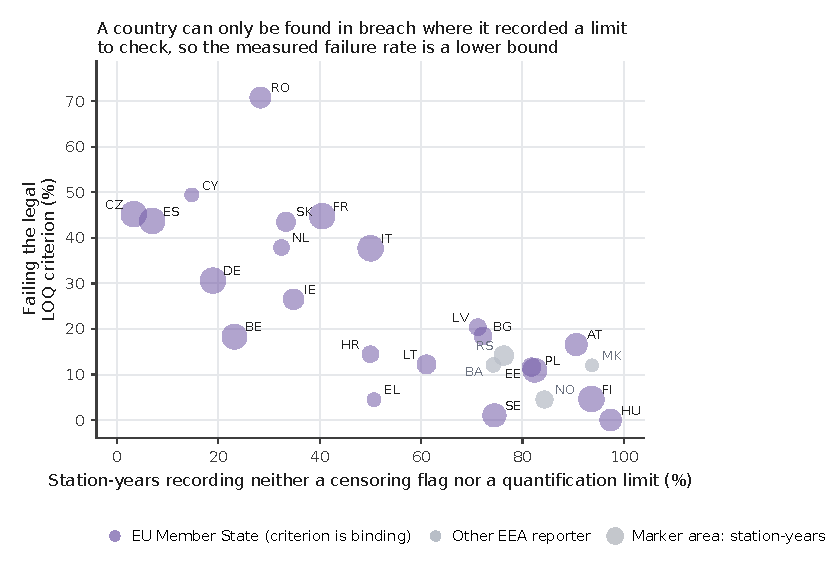
\includegraphics[width=0.86\textwidth]{fig03_country_practice.pdf}
\caption{Each point is a reporting country with at least \num{5000}
station-years; area is proportional to that count. The relationship runs the
wrong way for a chemical explanation: authorities recording least (right) are
found in breach least (bottom), because a limit that was never reported cannot
be tested against the standard. This is not a correlation between two
independent quantities and is not offered as one --- the horizontal axis governs
the \emph{denominator} of the vertical one, so the downward slope is the
signature of that dependence rather than a finding about chemistry. What it
establishes is one thing: the measured failure rate is a lower bound, and it is
loosest exactly where reporting is worst. Generated by \texttt{scripts/90\_figures.py}.}
\label{fig:country-practice}
\end{figure}

\paragraph{More than a third of European monitoring fails the legal
performance criterion.}
Article~4(1) of Directive 2009/90/EC requires a limit of quantification at or
below \num{30}\,\% of the relevant environmental quality standard before a
method's results may be used~\cite{eu2009qaqc}. \textbf{\num{40.1}\% of station-years assessed under a European standard were produced by a method that
does not meet it.}

\paragraph{Article~3(3b) is routinely unenforceable.}
Of the station-years for which a European standard exists, \textbf{\num{17.5}\% report a below-quantification result whose limit exceeds that standard}, which the Directive
requires to be set aside. For three pyrethroid insecticides --- deltamethrin,
bifenthrin and esfenvalerate --- the figure is \num{100}\%: none has ever, in
this record, been measured by a method capable of deciding its own standard.
Figure~\ref{fig:loqeqs}a ranks substances by the stricter Article~4(1)
criterion, on which a fourth --- clothianidin, a neonicotinoid --- also reaches
\num{100}\,\%.

\paragraph{The failure scales with the standard, not with the substance.}
The substances in Figure~\ref{fig:loqeqs}a share no chemistry, only the
\emph{magnitude of the limit written for them}. By decade of the
annual-average standard, the share whose quantification limit exceeds it rises
from \num{0.6}\,\% at order \num{10}~\si{\micro\gram\per\litre} to
\num{81.8}\,\% at \num{e-4}~\si{\micro\gram\per\litre}, over decades
carrying between \num{5} and \num{16} substances each
(Figure~\ref{fig:loqeqs}b). The two decades below that reach \num{100}\,\%
but rest on four substances and on one, so the trend is read from the decades
that can carry it.
Directive~(EU) 2026/805 moves the analyte list into exactly those decades:
\num{8} of the \num{24} substances it adds with an annual-average standard
put it below \num{e-3}~\si{\micro\gram\per\litre}
(\num{33}\,\%), against \num{7} of \num{35} on the legacy list
(\num{20}\,\%). The defect therefore grows unless analytical capability moves
down with the threshold, and nothing in the record suggests it has.

\begin{figure}[htbp]\centering
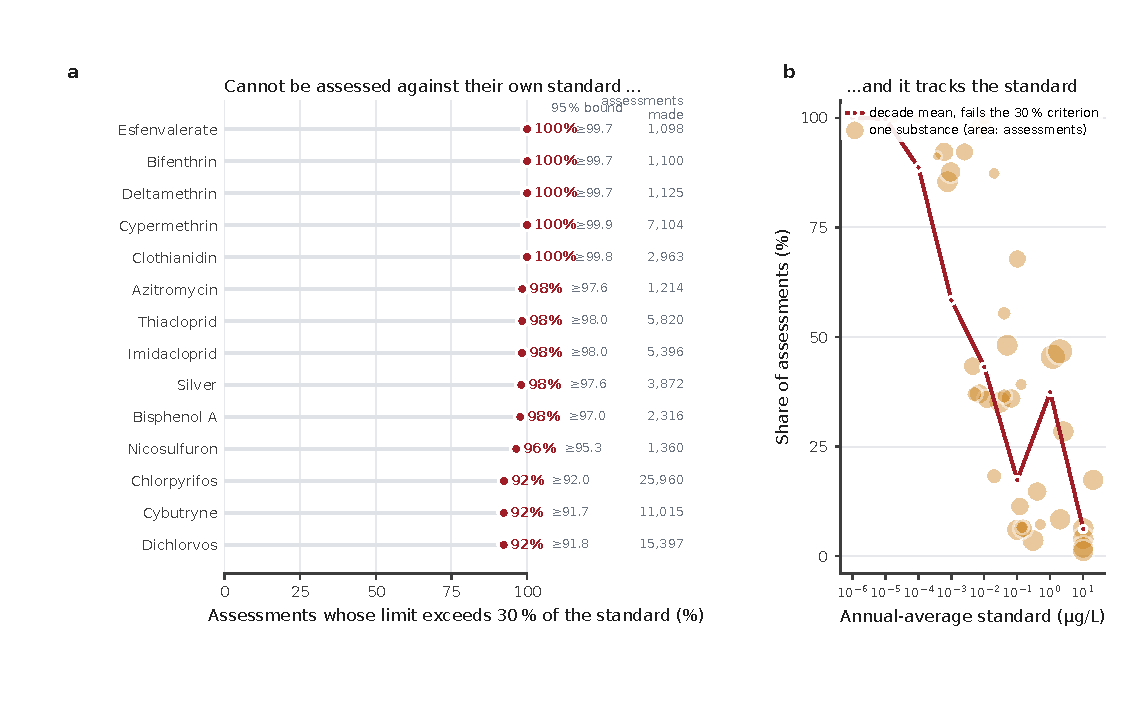
\includegraphics[width=0.86\textwidth]{fig04_loq_vs_eqs.pdf}
\caption{\textbf{(a)} The \emph{fourteen} substances with the highest share of
station-years whose quantification limit exceeds \num{30}\,\% of the
environmental quality standard, among those with at least \num{1000} assessable
station-years and at least one such station-year. The substances are selected
\emph{by} the quantity plotted, so the shaded band is the \num{95}\,\% Wilson
interval: ranking puts the least certain estimates on show, and the band is what
separates a substance assessed \num{25960} times from one assessed \num{1098}
times. Every substance meeting the criterion is in
\texttt{supplementary/figure\_data/fig04\_loq\_vs\_eqs.csv} with its interval,
and a column recording which were plotted. \textbf{(b)} The same failure against
the \emph{magnitude} of the standard rather than the identity of the substance,
over every decade holding at least \num{500} assessable station-years: the lower
the limit the law writes, the less often the monitoring can decide it. Between
\num{5} and \num{16} substances stand behind each decade from
\num{e1} down to \num{e-4}~\si{\micro\gram\per\litre}; the two lowest are
thin, and the circled point is a decade holding \emph{one} substance, whose rate
is that substance's rate and not a property of the decade. The composition of
every decade ships beside the figure. Generated by
\texttt{scripts/90\_figures.py}.}
\label{fig:loqeqs}
\end{figure}

\subsection{The record is not one era, and the three failures do not move together}
\label{sec:results-era}
Every row carries its own reference year, so the audit can be read year by
year\src{scripts/22\_waterbase\_external.py}. \num{48.8}\,\% of the river
record is dated \num{2015} or later, and the three failures behave differently
over time --- but not in the same way, and not gradually
(Figure~\ref{fig:by-year}).

\textbf{One failure was repaired on a date.} The share of station-years
declaring neither a censoring flag nor a limit falls from \num{31.8}\,\% in
\num{2012} to \num{0.0}\,\% in \num{2013}, and stays there for the
\num{12} years to \num{2024}: not a trend, a step. \textbf{The other two did
not move.} The share of assessments from a method failing the \num{30}\,\%
criterion is \num{46.3}\,\% in \num{2006} and \num{47.7}\,\% in
\num{2024}; the share whose limit exceeds the standard outright, \num{28.1}\,\%
and \num{28.2}\,\%. Substitution at source never moves at all: censored rows
carrying a positive value stay between \num{97.2}\,\% and \num{100}\,\%
across every year the record can speak about. Twelve years after the
record-keeping defect was repaired, the analytical defect is where it was.

\paragraph{The recent record is the stronger case, not the weaker one.} Before
\num{2013} an objection was available: the failures might be artefacts of
incomplete reporting. After it that objection is gone --- every station-year
carries its limit --- and the analytical failure is unchanged. Read on
\num{2024} alone, the last year in the record, \num{47.7}\,\% of assessments
still come from a method failing the performance criterion and \num{28.2}\,\%
from one whose limit exceeds the standard outright. What the paper reports is
therefore not a defect of an archive.

\begin{figure}[htbp]\centering
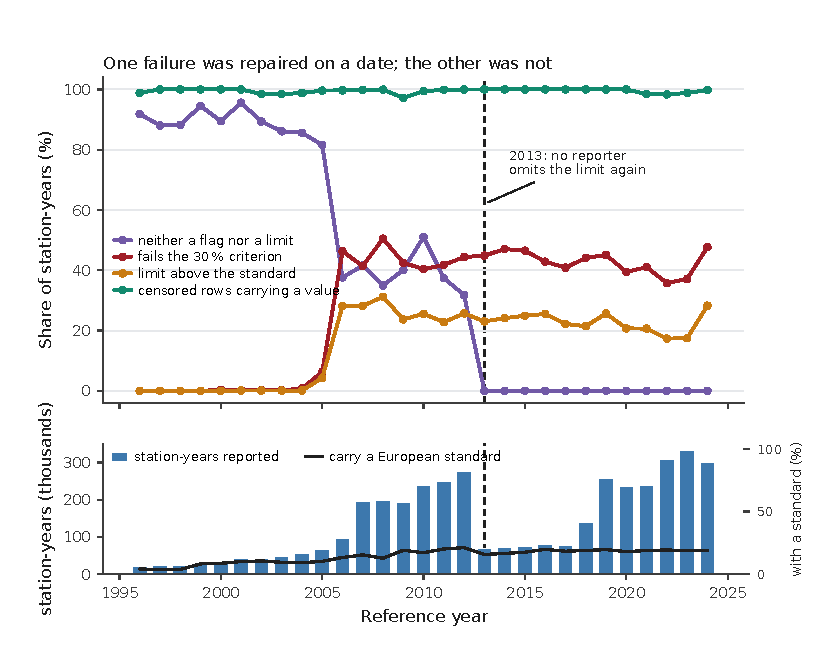
\includegraphics[width=0.86\textwidth]{fig08_by_year.pdf}
\caption{\textbf{(a)} The three failures by reference year, over the
\num{29} years holding at least \num{20000} station-years. The dashed line is
read from the data, not chosen: it marks the first year after which no reporter
omits the limit again. \textbf{(b)} The denominator, without which panel (a)
misleads: before \num{2005} almost no row carries a limit, so the legal criteria
read \num{0}\,\% for want of anything to test rather than because the
monitoring met them. Every year, plotted or not, is in
\texttt{supplementary/figure\_data/fig08\_by\_year.csv}. Generated by
\texttt{scripts/90\_figures.py}.}
\label{fig:by-year}
\end{figure}

Splitting at \num{2015} rather than at the break keeps the comparison
conservative and lets it be read against the era table
(Table~\ref{tab:era}).

\begin{table}[htbp]\centering
\caption{The audit split at \num{2015}. Shares of station-years, except the
legal criteria, which are over station-years for which a European standard
exists, and substitution, which is over censored rows. Full table in
\texttt{supplementary/S10\_by\_era.csv}, and by reporting country in
\texttt{S11\_era\_by\_country.csv}.}
\label{tab:era}
\begin{tabular}{lrr}
\toprule
 & before \num{2015} & \num{2015} onwards \\
 & (\num{2147102}) & (\num{2043731}) \\
\midrule
neither a censoring flag nor a limit & \num{49.7}\,\% & \num{0.0}\,\% \\
quantification limit above the standard & \num{22.7}\,\% & \num{21.8}\,\% \\
fails the \num{30}\,\% performance criterion & \num{38.5}\,\% & \num{41.4}\,\% \\
censored rows carrying a positive value & \num{99.6}\,\% & \num{99.3}\,\% \\
\bottomrule
\end{tabular}
\end{table}

\textbf{The record-keeping failure is solved}: station-years declaring neither
a flag nor a limit fall from \num{49.7}\,\% to \num{0.0}\,\%. \textbf{The
analytical failure does not move.} Its earlier figure is lower only because so
little of the old record can be tested: where no limit was recorded, no method
can be found wanting, so the rate is a lower bound.
\textbf{Substitution at source has not moved at all}: \num{99.3}\,\% of
censored rows still carry a positive number in place of the non-detection.

\paragraph{The fall is practice, not composition.} The set of reporters differs
between the periods, so a falling rate proves nothing on its own. The \num{8}
authorities reporting in both go to \num{0.0}\,\%, Denmark from \num{88.1}\,\%
(\texttt{supplementary/S11\_era\_by\_country.csv}), with no change to the
standard they report under.

\paragraph{What this does not license.} Those \num{8} are the only authorities
with a post-\num{2015} river record here, and \num{29} of the \num{37}
reporters have none, so any statement about \emph{current European practice}
rests on a handful of programmes. What holds without qualification is narrower:
where the record-keeping defect was repaired, the reporter repaired it, and the
analytical defect survived the repair.

\subsection{Two modelling choices the record decides}
\label{sec:results-modelling}
The record decides two commitments from Section~\ref{sec:methods-vocab} that
separate CENSO from the vocabularies in
Section~\ref{sec:results-gap}\src{scripts/22\_waterbase\_external.py}: where
the quantification limit lives, and what a standard written over a sum means.

\paragraph{The limit is not a property of the instrument.}
If it were, the same substance at the same station would carry the same limit
each year. Of the \num{557956} station--substance pairs reported in more than one
year, \textbf{\num{56.4}\,\% report more than one limit}. Whether the method
changed with it cannot be read from the record: only \num{13654} of those pairs
--- \num{2.4}\,\% --- report an analytical method code at all, and \num{3356}
of those that do report more than one. In \textbf{\num{21043} pairs the change
crosses the standard}: the same station and substance is decidable in one year
and not the next. A vocabulary that binds the limit to a sensor cannot express
that; one that binds it to the run at least has somewhere to put the provenance
this record is missing.

\paragraph{A sum standard is not a limit on any of its members.}
Annex~I states four limits over a group rather than a substance --- a
component-based standard resting on concentration
addition~\cite{backhaus2012mixtures,posthuma2019mixtures} --- and a sum from an
incompletely measured basket is an underestimate the arithmetic never reveals;
CENSO carries \texttt{requiresCompleteGroup} for it. All four resolve from the
Annex, and the completeness rate falls with the size of the basket: heptachlor
and its epoxide (\num{2} members) are both measured in \num{69.6}\,\% of the
station-years that touch them, the cyclodiene pesticides (\num{4}) in
\num{88.0}\,\%, the polyaromatic hydrocarbons (\num{9}) in \num{36.0}\,\%
--- and the sum over the pesticides list, which resolves to \num{75} members,
in \textbf{\num{0.0}\,\%}: not one of the \num{26846} station-years that
touch that group measures all of it. A standard defined over seventy-five
substances that no station-year ever measures completely cannot be assessed by
anyone, and a threshold column would compare the partial sum against it and
return compliance.

\subsection{The ontology applied to open data}
\label{sec:results-wbabox}
Expressing a Waterbase subset in CENSO\src{scripts/23\_waterbase\_abox.py}
tests whether its distinctions survive a schema written by someone else: every
class is assigned from EEA columns.

\paragraph{The assessment is the population, not a sample.}
The decision is arithmetic on four reported fields, applied to all
\num{696168} station-years whose substance carries a European
standard\src{scripts/22\_waterbase\_external.py}. \textbf{\num{43.8}\,\% are not
decidable from the record as reported} --- one outcome,
\texttt{IndeterminateCompliance}, reached for four distinct reasons the
vocabulary keeps apart as its subclasses: \num{18.8}\,\%
\texttt{PreconditionUnmet}, where the standard is defined on a quantity the
record does not report (Section~\ref{sec:results-precondition});
\num{17.5}\,\% \texttt{MethodInsufficient}, where a below-quantification result
carries a limit above the standard, which Article~3(3b) requires to be set
aside; \num{6.5}\,\% \texttt{BoundNotEstablished}, with no bound to compare at
all; \num{1.0}\,\% \texttt{PossibleExceedance}, where the interval straddles the
limit. A two-valued schema has nowhere to put any of them and collapses all four
into compliance.

The taxonomy is not free ornament, and the cheaper alternative shows why: a
schema with a single indeterminacy flag reports the same \num{43.8}\,\% and
loses the four. They are not degrees of one defect but different objects, and
they call for different repairs --- a schema field for the covariates, a better
laboratory, a reported limit, a reported uncertainty --- of which only one is
addressed by anything an analyst can do to the data afterwards.

\paragraph{One reason comes from the standard rather than from the record.}
\texttt{PossibleExceedance} requires an interval around a quantified result,
and no European release reports a per-result measurement uncertainty,
aggregated or disaggregated. Article~4(1) caps that uncertainty at
\num{50}\,\% ($k=2$) at the level of the standard, so the widest lawful
interval around a reported value $x$ is $x \pm 0.5\,T$, straddling the
standard when $0.5\,T < x < 1.5\,T$ --- a band around $T$, not an
extrapolation. What is reported is a bound, not an estimate.

\paragraph{What a two-valued pipeline reports for the same rows.}
Entering a non-detection at half its quantification limit is not a convention an
analyst chose. Article~5(1) of Directive 2009/90/EC requires it: ``where the
amounts of physico-chemical or chemical measurands in a given sample are below
the limit of quantification, the measurement results shall be set to half of the
value of the limit of quantification concerned''~\cite{eu2009qaqc}. The same
instrument that sets the performance criterion also mandates the substitution,
and the substitution pushes results \emph{above} the standard: of the \num{171285}
exceedances such a pipeline reports, \num{112034} exist only because the
substitution lifted a censored result past the limit, \num{30140} are asserted
against a standard that is not defined on the quantity the record reports, and
\num{12142} rest on a number whose censoring status the record never states.
\num{14505} are exceedances the law can affirm --- quantified, above the
standard, with an applicable standard and an interval that does not straddle it.
A further \num{2458} are quantified above the standard and set aside all the
same, because the widest interval Article~4(1) permits straddles it. Article~3(3b)
sets aside no quantified result: it reaches a value reported as below the
quantification limit, and a mean quantified above the standard is evidence of
exceedance whatever the method's limit was. Zero, half the limit and the limit
itself report \num{59251}, \num{171285} and \num{200708} exceedances over the
same records --- a \num{3.4}-fold range in the enforcement-relevant number,
selected by a rule the data does not determine
(Figure~\ref{fig:verdicts}).

\paragraph{The graph is a materialisation, not the analysis.}
A reservoir sample of \num{40000} station-years is expressed as RDF
(\num{501062} triples): a pure-Python triple store cannot hold four million
rows, and inflating it would misreport what was reasoned over. \num{11.7}\% of
its observations are \texttt{UnresolvedObservation}, a state no other surveyed
vocabulary can express.

\begin{figure}[htbp]\centering
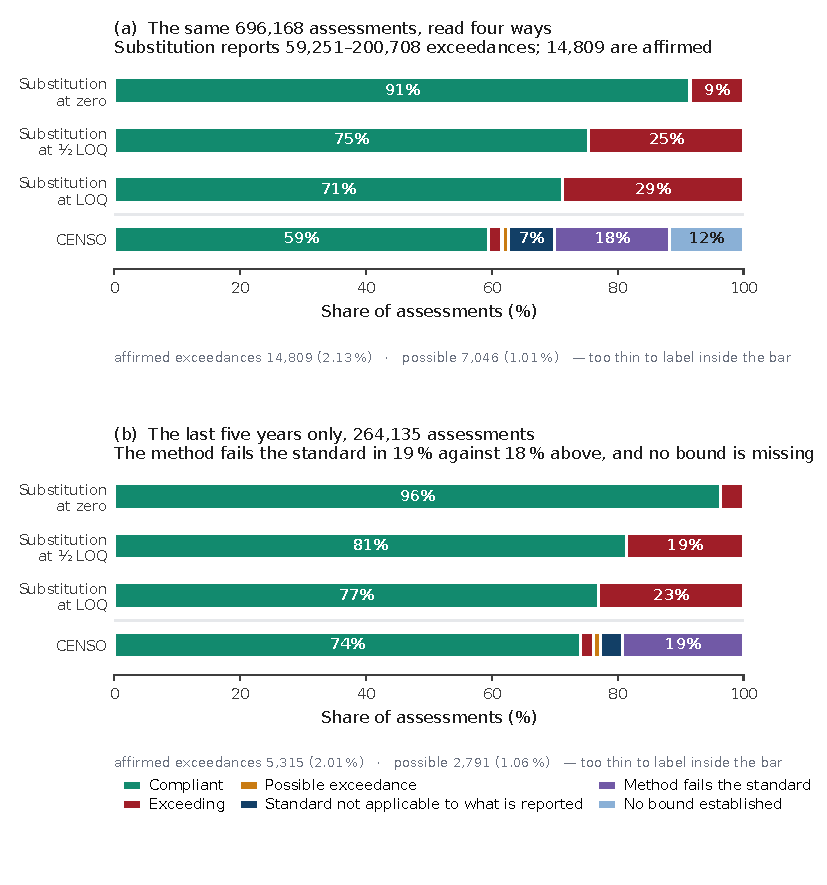
\includegraphics[width=0.86\textwidth]{fig05_verdicts.pdf}
\caption{The same \num{696168} assessments --- every station-year whose
substance carries a European standard, not a sample --- read four ways. The top
three rows are the identical records under the three substitution conventions
in routine use; they disagree about the number of exceedances by a factor of
\num{3.4}, and \num{14505} are exceedances the law can affirm. The bottom
row reports the outcomes the law distinguishes instead of absorbing them into
compliance; \emph{possible exceedance} is a quantified result whose widest
lawful uncertainty interval straddles the standard. The plotted values are in
\texttt{supplementary/figure\_data/fig05\_verdicts.csv}. Generated by
\texttt{scripts/90\_figures.py}.}
\label{fig:verdicts}
\end{figure}

\paragraph{What the graph adds, and what it does not.}
The graph returns the same method-insufficiency share as the streaming count
--- \num{17.2}\,\% on the sample against \num{17.5}\,\% on the population,
inside the \num{0.19}-point sampling error --- but that agreement is a
consistency check rather than corroboration: both routes call one decision procedure, held in a single module
precisely so the two cannot drift. What the check establishes is that
expressing the record in the vocabulary loses nothing --- every row classified
in RDF lands where the counter puts it. What it does not establish is that the
ontology was needed to count: it was not. The counting could always have been
done. What only the graph does is answer \emph{which} assessments are
unsupportable, under which limit, for which substance, in one query.

\subsection{A standard that cannot be applied to what the record reports}
\label{sec:results-precondition}
Two Annex~I footnotes make a threshold conditional rather than absolute. Footnote
12 states that the standards for lead and nickel ``refer to bioavailable
concentrations of the substances''; footnote 9 that cadmium's ``vary depending on
the hardness of the water as specified in five class categories''. Bioavailable
normalisation needs hardness, dissolved organic carbon and pH; the hardness class
needs hardness. WISE-6 reports none of them on the row.

So for these three substances there is no comparison to make. Not a strict one
and not a lenient one: the number in Annex~I and the number in the record are not
measurements of the same quantity, and asking whether the method's limit reaches
\num{30}\,\% of the standard is asking about the wrong quantity. The released
package attaches the two conditions to the six thresholds they govern, and the
assessment returns \texttt{PreconditionUnmet} ahead of every other test ---
before the value, before the limit, before Article~3(3b).

\textbf{That is \num{131068} assessments, \num{18.8}\,\% of every station-year
a European standard reaches}\src{scripts/22\_waterbase\_external.py}. They are
not a marginal stratum: cadmium, lead and nickel are among the most reported
substances in the record. A two-valued pipeline decides all of them anyway, and
decides them in both directions --- \num{30140} are reported as exceedances of a
standard that is not defined on what was measured, the remainder as compliance
with it.

This is the commitment a threshold column cannot hold at all. The other three
could in principle be bolted onto a table: a censoring flag, a limit per row, a
verdict enumeration. A precondition is a property of the \emph{standard} --- it
travels with the regulation, not with the measurement --- so a column of
thresholds has nowhere to record that a threshold was inapplicable, and no way to
distinguish that from a threshold that was met. The vocabulary named lead, nickel
and cadmium in its class comments before this record was read; the record returns
\num{131068} assessments where those comments decide the outcome.

This stratum is metals, and only metals, because Annex~I attaches its
applicability conditions there and nowhere else. It is one of the four reasons an
assessment can be undecidable, not the paper's subject: censoring itself is far
worse among the organic micropollutants, where over three-quarters of samples
fall below the limit against under half for the Annex~I metals
(Section~\ref{sec:disc-lipinski}), and where the substances the record can least
often decide --- pyrethroids, neonicotinoids, pharmaceuticals, bisphenol~A ---
are concentrated (Figure~\ref{fig:loqeqs}a). A condition on the analysed
fraction would reach every metal rather than three: Article~3(1) defines the
metal standards on the dissolved phase and WISE-6 reports the analysed matrix,
so such a condition would be checkable in both directions rather than merely
unsatisfiable. The vocabulary does not declare one, because no footnote in the
consolidated Annex~I creates it and a class no package can instantiate is a
promise rather than a term; it is the next thing the machinery should decide.

\subsection{The substitution has already happened before anyone downloads
the data}
\label{sec:results-asreported}
Sections~\ref{sec:results-waterbase} and~\ref{sec:results-wbabox} treat
substitution as something an analyst does to a record. The ontology's SHACL
shapes, run over the record \emph{as reported} with none of our pipeline's
repair\src{scripts/26\_source\_conformance.py}, show that it is not.

\textbf{\num{55.0}\% of river station-years declare a result below the limit of
quantification and, in the same row, state a positive value for it.} A
non-detection permits any concentration down to zero; a positive lower bound is
a number someone chose, and the reporting authority chose it before
publication. Counted over the censored rows alone rather than over the whole
record, the share is \num{99.4}\,\%: where a row is flagged at all, it almost
always carries a substituted number as well.

This changes who the finding is about. Where the flag survives, as in
Waterbase, the substitution is visible and can be undone, which makes the
counterfactual in Section~\ref{sec:results-wbabox} computable. Where it does
not --- \num{25.5}\% of the record, by Section~\ref{sec:results-waterbase} ---
the same substitution cannot be detected, let alone reversed.

\paragraph{The shapes are the deliverable, not the demonstration.}
A deterministic sample of \num{20000} concentration rows validated against the
published shapes yields \textbf{\num{14137} violations}, all of one kind: a
result below the quantification limit carrying a positive number for it. A
published constraint catches the substitution, not a bespoke script.

An earlier version of the shapes required every method to state a limit of
\emph{detection}, so they fired on every row: WISE-6 has no field for one, and
Article~3(3b) of Directive 2008/105/EC and Article~4(1) of Directive 2009/90/EC
are written about the quantification limit. Our own graph satisfied that
constraint by manufacturing the datum at $\mathrm{LOD}=\mathrm{LOQ}/3$. The
shapes now require \emph{a} limit, and the ABox states the one the source
reports. The distinction the old constraint reached for is real and is made in
Section~\ref{sec:methods-noise}: a non-detection establishes
$[0,\mathrm{LOD}]$, the record at best $[0,\mathrm{LOQ}]$, a weaker and
different claim.

\subsection{The same observations under two regulations}
\label{sec:results-dual}
Pluggable regulation packages let one set of observations be assessed under
several jurisdictions without
reimplementation\src{scripts/24\_dual\_regulation.py}, as
Section~\ref{sec:methods-why} claims: both packages are read as data, and only
the file supplying the threshold changes.

Of the \num{1488677} river station-years regulated by at least one instrument,
\num{81.9}\% change outcome when the package is swapped, but most of that is
coverage: one jurisdiction regulating a substance the other does not, a fact
about the legal texts rather than about any measurement. Where \emph{both}
regulate and only the numeric standard differs, \textbf{\num{17.7}\% (95\,\% CI \num{17.6}--\num{17.9}\,\%) still change outcome}, mostly the \num{47999} the
European standard sets aside as method-insufficient and the looser Turkish
limit can decide.

An assessment that is \emph{method-insufficient} under one instrument and
decidable under another is not expressible if the threshold is a column:
method adequacy is a relation between the limit and the standard. Both verdicts
can be held at once, on thresholds with different IRIs, and neither overwrites
the other. Turkish standards are not in force over European rivers; the
comparison is counterfactual by construction and demonstrates that the
machinery is regulation-independent, never that it assesses Türkiye.

\subsection{A standard defined on a different unit of observation}
\label{sec:results-mac}
Annex~I states two standards for most priority substances: an annual average,
defined against an annual mean, and a maximum allowable concentration, defined
against an \emph{individual measurement}. Everything above evaluates the first,
on the aggregated release, where one row \emph{is} an annual mean. The second
could be approached there --- the release carries an annual maximum --- but not
answered: that column is absent for part of the record, carries its own
below-quantification flag for less of it, and gives no per-sample denominator,
so the share of samples a method cannot decide is not recoverable from it. The
vocabulary holds the two standards apart, and conflating them is an
inconsistency.

Reading the disaggregated release --- \num{96597294} individual sample records
--- makes it computable\src{scripts/27\_mac\_exceedance.py}. Of the \num{8148785}
river samples with such a standard and a convertible unit, \num{74702} exceed it outright and \textbf{\num{794418} (\num{9.7}\,\%) are undecidable}: not
detected, with a quantification limit \emph{above} the standard, so no result
the method could have returned would have settled it. Article~3(3b) requires
those to be set aside; a two-valued pipeline records every one as compliant.

\paragraph{The two standards disagree, and a column can hold only one.}
Of the \num{66285} station-years assessable under both,
\num{25.6}\,\% receive different verdicts: in \textbf{\num{1.1}\,\% --- \num{698} station-years --- the published annual mean is compliant while
a sample behind it breaches the maximum allowable concentration}
(Figure~\ref{fig:two-thresholds}a), in the rest the mean exceeds while no
single sample does. Neither verdict is wrong and neither supersedes the other;
Annex~I asks both. A schema storing one threshold per substance cannot record
which it holds.

\begin{figure}[htbp]\centering
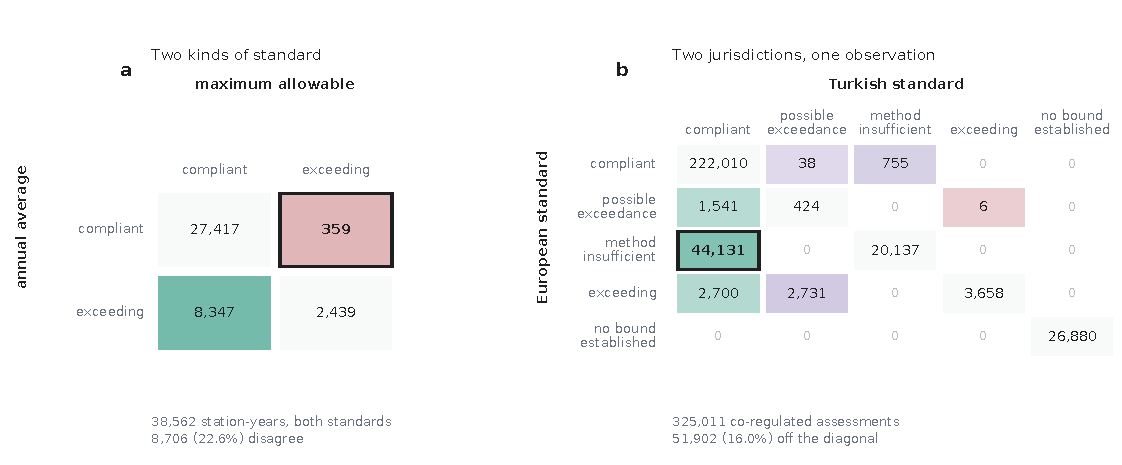
\includegraphics[width=\textwidth]{fig07_two_thresholds.pdf}
\caption{What a threshold column cannot hold, on real observations. Each panel
cross-tabulates the same observations assessed twice; grey is agreement, colour
is the verdict the second assessment changes \emph{into}, and the outlined cell
is the one the text names. \textbf{(a)} The same station-year under the two
standards Annex~I states for it: an annual average, on the published mean, and
a maximum allowable concentration, on the samples behind that mean.
\textbf{(b)} The same observation under two jurisdictions' packages; the
Turkish standards are not in force over European rivers, so this demonstrates
the machinery rather than assessing either jurisdiction. Its
\emph{no bound established} row and column are empty except on the diagonal,
and that is the result rather than an artefact: a record that establishes no
bound establishes none under either instrument, so the one outcome that cannot
move is the one caused by the reporting rather than by the law. The plotted counts are
in \texttt{supplementary/figure\_data/fig07\_two\_thresholds.csv}. Generated by
\texttt{scripts/90\_figures.py}.}
\label{fig:two-thresholds}
\end{figure}

The disaggregated release does not hold the samples behind every aggregated
station-year, so these shares describe the stratum readable at both units and not
the whole record: \num{66285} of the \num{376843} station-years that carry an
annual-average verdict and a maximum-allowable standard --- \num{17.6}\,\% ---
have samples behind them in the disaggregated release. Whether that stratum
resembles the rest is not something the release lets us test, since the missing
station-years are missing precisely their samples; the per-substance and
per-country coverage is in
\texttt{supplementary/S12\_mac\_exceedance.csv} so a reader can see which
substances it rests on. A censored sample is decided
by its quantification limit, never by the number the reporter wrote in its
place, the artefact Section~\ref{sec:results-asreported} exposes.

\subsection{Is the between-country spread an artefact?}
\label{sec:results-confounders}
The share of station-years carrying neither a censoring flag nor a limit ranges
from \num{3.3}\% to \num{97.4}\% between countries reporting under the same
directive (Figure~\ref{fig:country-practice}). The countries differ in
substances, years and Member State status, so the objection is
testable\src{scripts/25\_country\_confounders.py}. WISE-6 defines the field
identically for every reporter, and a national standard changes which results
breach a limit, not whether the limit was written down. Three adjustments ---
the pooled European substance mix, the substances most of these countries
report, and EU membership --- each leave the spread intact, with
Kendall's~$\tau$ between the raw and standardised orderings at \num{0.89};
per-country values are in supplementary table~S5. Restricting to recent years,
in Section~\ref{sec:results-era}, is not a fourth test, because too few
countries report after \num{2015}. A spread stable under three independent
corrections is a property of reporting practice.

\subsection{Comparison with published ontologies}
\label{sec:results-gap}
% generated by scripts/07_verify_gap_table.py
% GENERATED by scripts/07_verify_gap_table.py -- do not edit.
\begin{table*}[htbp]\centering
\caption{Concepts present in published water and observation ontologies, decided by parsing each ontology file rather than its documentation. A dash means the file parsed and the concept was absent; \texttt{?} means it could not be retrieved, and no claim is made. The \emph{LOD bound to} column is the discriminating one: a detection limit declared as a sensor capability cannot state that a given measurement fell below it. The two rows marked \emph{this work} are CENSO's own modules and are not among the assessed vocabularies, which is why the text counts eighteen where the table has twenty rows.}
\label{tab:gap}
\scriptsize\setlength{\tabcolsep}{3.5pt}
\begin{tabular}{l r l cccccc}
\toprule
Ontology & Ent. & LOD bound to & det.\ limit & censoring & undecid. & threshold & interval & applic. \\
\midrule
SOSA/SSN & 37 & -- & -- & -- & -- & -- & -- & -- \\
SOSA core & 53 & -- & -- & -- & -- & -- & -- & -- \\
GeoSPARQL & 0 & -- & -- & -- & -- & -- & -- & -- \\
QUDT schema & 239 & -- & -- & -- & -- & \checkmark & -- & \checkmark \\
SAREF core & 131 & -- & -- & -- & -- & \checkmark & -- & -- \\
SAREF4WATR v2.1.1 & 95 & -- & -- & -- & -- & \checkmark & -- & -- \\
SSN-system & 44 & the sensor & \checkmark & -- & -- & -- & -- & -- \\
OWL-Time & 78 & -- & -- & -- & -- & -- & -- & -- \\
WHOW water-monitoring & 57 & -- & -- & -- & -- & -- & \checkmark & -- \\
DoCE (Rio Doce WQ) & 168 & -- & -- & -- & -- & -- & -- & \checkmark \\
InWaterSense core & 189 & -- & -- & -- & -- & \checkmark & \checkmark & -- \\
InWaterSense regulations & 144 & -- & -- & -- & -- & -- & -- & -- \\
InWaterSense pollutants & 9 & -- & -- & -- & -- & -- & -- & -- \\
WAM-ONTO & 921 & -- & -- & -- & -- & -- & -- & -- \\
SewerNet & 145 & -- & -- & -- & -- & -- & -- & -- \\
CHMO (chemical methods) & 3438 & the method & \checkmark & -- & \checkmark & -- & \checkmark & -- \\
AFO (Allotrope) & 3864 & -- & -- & -- & -- & \checkmark & \checkmark & \checkmark \\
STATO (statistics) & 1162 & -- & -- & -- & -- & \checkmark & \checkmark & -- \\
ENVO & 7208 & -- & -- & -- & -- & -- & -- & -- \\
ExO (exposure) & 195 & -- & -- & -- & -- & -- & -- & -- \\
\textbf{CENSO (this work)} & 50 & \textbf{the result} & \checkmark & \checkmark & \checkmark & \checkmark & \checkmark & \checkmark \\
\textbf{CENSO-REG (this work)} & 17 & -- & -- & -- & -- & \checkmark & -- & -- \\
Project ontology 2018 & 123 & unclear & \checkmark & -- & -- & -- & -- & -- \\
\bottomrule
\end{tabular}
\end{table*}

\num{21} ontology files were assessed by parsing each one rather than reading
its documentation\src{scripts/07\_verify\_gap\_table.py}: \num{20} published
vocabularies plus one unpublished domain ontology as a non-standard baseline
(Table~\ref{tab:gap}). The set deliberately reaches outside the water domain.
CENSO claims applicability to any measurement process with a detection limit,
and a domain-independence claim tested inside one domain is not tested, so the
comparison includes the vocabularies built for the laboratory --- CHMO, the
\textsc{obo} Chemical Methods Ontology; AFO, the Allotrope Foundation Ontology,
built by a pharmaceutical consortium for analytical instrument data; and STATO,
the \textsc{obo} statistics ontology, where censoring is a routine concept in
survival analysis.

\textbf{No ontology except CENSO carries a censoring status.} That column is
empty for all \num{21}, and it is the one the argument rests on. It is also the
column the matcher was made hardest to fail: the patterns admit
\emph{censored}, \emph{left-censored}, \emph{right-censored},
\emph{left-truncated}, \emph{non-detect}, \emph{not detected},
\emph{not quantifiable} and \emph{below \dots\ limit} bare, and STATO --- where
censoring is routine in survival analysis --- declares no term for it and does
not mention it in a single definition. One ontology besides CENSO scores for a
not-determinable outcome, and it should not: CHMO's two hits are
\texttt{ambiguous synonym}, an \textsc{obo} annotation property describing the
quality of a synonym, and \texttt{double quantum transitions for finding
unresolved lines}, a technique in which the unresolved things are spectral
lines. The cell is left standing and the discrepancy published beside the table,
because a pattern narrowed until a competitor loses a cell would make the
comparison an assertion again.

\paragraph{The patterns are deliberately generous, and the asymmetry is the
point.} Every widening can only add a \emph{yes} to a competitor's row: CENSO's
own cells are already filled, so no adjustment to the matcher can flatter this
work. The lists were widened after the first version was found to match on our
vocabulary's spellings and miss other people's --- it did not match
\emph{limit of quantitation}, the pharmacopoeial spelling a laboratory ontology
is most likely to use, nor \emph{below detection limit}, the most ordinary
phrasing there is, nor \emph{minimum value} spelled out. A claim that survives a
matcher tuned in the competitors' favour is worth something; one that depends on
spelling is not.

Two columns need reading carefully, because a keyword match is not a modelling
commitment. Two vocabularies score for an interval-valued result, but only WHOW
attaches the interval to the \emph{result}: InWaterSense's range properties
describe the range a \emph{device} can report, and AFO's \texttt{lower bound}
and \texttt{upper bound} are subclasses of \texttt{bound role} --- roles borne
by a participant, with no property placing an interval on a measured datum.
Those cells are left scored, and the discrepancy published beside the table
rather than corrected away: a pattern adjusted until a competitor scores the way
we want would make the table an assertion again.

\paragraph{The sharpest case is CHMO, and it is not a water ontology.}
\textbf{CHMO declares \texttt{limit of detection} (CHMO:0002801) and
\texttt{limit of quantification} (CHMO:0002802), both defined from the IUPAC
Gold Book} --- so the gap is not that chemistry lacks the concept. CHMO binds
them to the \emph{method}, as a \texttt{figure of merit} of an assay:

\begin{center}
\texttt{limit of detection} $\sqsubseteq$ \texttt{figure of merit} $\sqsubseteq$
\texttt{assay output} $\sqsubseteq$ \texttt{data entity}
\end{center}

\noindent That is a better place than SSN-system's, which makes the limit a
\texttt{SystemProperty} of a \emph{sensor}, and it is still not a place from
which any particular result can be called censored. None of CHMO's
object properties relates a limit to a result; they are the \textsc{bfo}/\textsc{ro}
relations (\texttt{has participant}, \texttt{is specified output of},
\texttt{has characteristic}). The limit is known about the assay and forgotten
about the measurement --- the same failure as the sensor case, one step closer.
This is the result we would most have expected to lose, and it is the reason the
claim is worth making: the concept exists, is well defined, is cited to the
IUPAC Gold Book, and still nothing can say that \emph{this} number is a bound.

Profiling for sampling versus sensing terminology separates the vocabularies
cleanly: SAREF core scores \num{0}/\num{22} sampling to sensing terms, CENSO
\num{3}/\num{0}. \textbf{The field is dominated by vocabularies built for
in-situ sensing}, in which a detection limit is properly a device property, and
the few sampling-aware ones carry no limits at all.

Five further ontologies described only in papers (WaWO+, OPO, InWaterSense's
expert system, Ahmedi et al., Acquirium) were assessed from their full
text\src{scripts/11\_assess\_competitor\_papers.py}: in none do \emph{detection
limit}, \emph{LOD}, \emph{LOQ}, \emph{censoring} or \emph{non-detection} occur.
This is weaker evidence than parsing a file and is labelled as such.

\subsection{What a term list cannot show: the vocabularies cannot separate the
readings}
\label{sec:results-separation}
A gap table records which vocabulary declares which term, and invites an
answer we think a referee is entitled to give: a missing term is a missing
convenience, not a missing capability, and anyone may mint a subclass. The
answer to that is logical rather than lexical. A vocabulary distinguishes two
situations only if some sentence it can write is true of one and false of the
other. So we take one real record, write down the readings it admits, and ask
of each vocabulary whether the readings it can \emph{express} still
differ\src{scripts/13\_separation.py}.

The witness is the row of Figure~\ref{fig:geometry}(b): imidacloprid at a
Spanish river station, reported below a quantification limit of
\num{0.01}~\si{\micro\gram\per\litre}, carrying \num{0.01} as its value,
against an annual-average standard of
\num{0.0068}~\si{\micro\gram\per\litre}. Nothing about it is constructed --- the
standard lies inside the censored interval, and the reported value is the limit
itself, which is what substitution at source looks like in this release. Those
four numbers admit three readings: the censoring is honoured and the result is
the interval $[0,\mathrm{LOQ}]$ (\textbf{R1}); the flag is dropped and the
number is a measurement, which a numeric comparison calls an exceedance
(\textbf{R2}); or the number arrives with neither flag nor limit, the
\num{25.5}\,\% case (\textbf{R3}). R1 and R2 are the pair the paper turns on:
the same four numbers, two different claims.

Each reading is translated into each vocabulary, generously: a fact survives if
the vocabulary has \emph{any} term in the concept family it needs, and every
vocabulary is granted an observation and a reported number without being
checked for them. The families are the gap table's own columns, so nothing is
decided here that parsing the files did not already decide.

\begin{quote}
\textbf{Proposition.} R1 and R2 differ only in facts whose families are
\emph{censoring}, \emph{interval-valued result} and \emph{undecidable verdict}.
A vocabulary declaring no term in those families translates both readings to
the same set of facts; hence for every sentence $\varphi$ in that vocabulary,
R1 entails $\varphi$ exactly when R2 does.
\end{quote}

\textbf{\num{20} of the \num{21} vocabularies collapse R1 into R2.} The one
exception is CHMO, and it is an artefact of the generous matcher rather than a
capability: CHMO is credited with a not-determinable outcome on the strength of
\texttt{ambiguous synonym} and \texttt{unresolved lines}, so R1 receives a
\texttt{no\_verdict} fact that R2 does not. Read strictly it collapses with the
rest, and it has no censoring term either way. We report the number the generous
matcher gives. For the other \num{20}, no query, rule or
reasoner built on them returns a different answer for a non-detection than for
a measurement at the same number --- not because none has been written, but
because none can be. SSN-system and the \num{2018} baseline separate R1 from
R3, but only by noticing that a limit was stated somewhere; neither can say
that \emph{this} result fell below it, which is what the discriminating column
of Table~\ref{tab:gap} records. Two vocabularies with interval-valued results,
WHOW and InWaterSense core, would separate R1 from R2 if the interval could be
asserted without a censoring term --- but that assertion has no ground in a
vocabulary with no term for the flag, which is the distinction at issue rather
than a counter-example to it. The sensitivity is reported in
\texttt{eval/separation.md} rather than left for a reader to raise.

The same three readings run through the reasoner against CENSO entail
\texttt{CensoredObservation} with \texttt{MethodInsufficient},
\texttt{QuantifiedObservation} with \texttt{Exceedance}, and
\texttt{UnresolvedObservation} with no outcome at all. The outcome is entailed
and not asserted: \texttt{Exceedance} is an equivalent class of an observation
bearing \texttt{exceeds} to a threshold. And the separation is a property of
the vocabulary rather than of the loader that populates it --- merging any two
readings of the same individual is an inconsistency, from the disjointness of
the detection statuses. A pipeline cannot quietly hold two readings of one
record.

None of this says the other vocabularies are wrong, or that they could not be
extended; any of them could be given a censoring class tomorrow. It says what
reuse as published currently supports, and where the distinction has to live
once it is added: on the result, not on the device.

\subsection{The ontology answers the questions it was built for}
\label{sec:results-cq}
Twenty competency questions, each tied to an axiom, were executed over the
Waterbase graph with the two vocabulary modules and both regulation packages,
\num{507708} triples as
loaded\src{scripts/17\_run\_competency\_questions.py}. \textbf{All twenty
return answers.} Full OWL~2~RL closure over a graph this size is impractical in
pure Python, so only two entailments are materialised: union membership for the
two defined observation classes, and \texttt{rdfs:subClassOf} on type
assertions. That is measured rather than asserted: over synthetic ABoxes on the
same vocabulary, closure time grows super-linearly in the number of
observations, because RL closure writes every entailment into the graph instead
of answering against rules; SHACL validation over the same graphs costs about an
order of magnitude less\src{scripts/14\_reasoning\_benchmark.py}. The series
is in \texttt{supplementary/S13\_reasoning\_cost.csv}. A deployment over a
whole basin would use a store with native rule support, so those figures bound
this pipeline and not the approach. Every other answer comes from asserted triples. They run on public
data, and their SPARQL, rows and times are in the supplementary material.

\subsection{Four real rows, decided twice}
\label{sec:results-walkthrough}
Figure~\ref{fig:walkthrough} takes one station-year from each of four outcome
classes and decides it twice: once by the vocabulary, once by a two-valued
pipeline at each of the three substitution constants in
use\src{scripts/92\_decision\_walkthrough.py}. The rows are the first match per
class in sorted order, so the selection cannot flatter the argument, and the
two-valued verdicts are computed by the same function that produces the counts
in Section~\ref{sec:results-wbabox} rather than by a second implementation.

\textbf{Two of the four get a different two-valued verdict depending on which
constant the pipeline happened to use}, and nothing in a two-valued output
records that a choice was made. Permethrin is the clearest: a quantification
limit of \num{0.02}\,\si{\micro\gram\per\litre} against a standard of
\num{0.00027} --- \num{74} times the threshold it was meant to decide --- reads
as compliant at zero and as exceeding at half. The first case is included
because both systems agree on it: a bound that clears the standard decides the
question, and a vocabulary that could not say so would be useless.

\begin{figure}[htbp]\centering
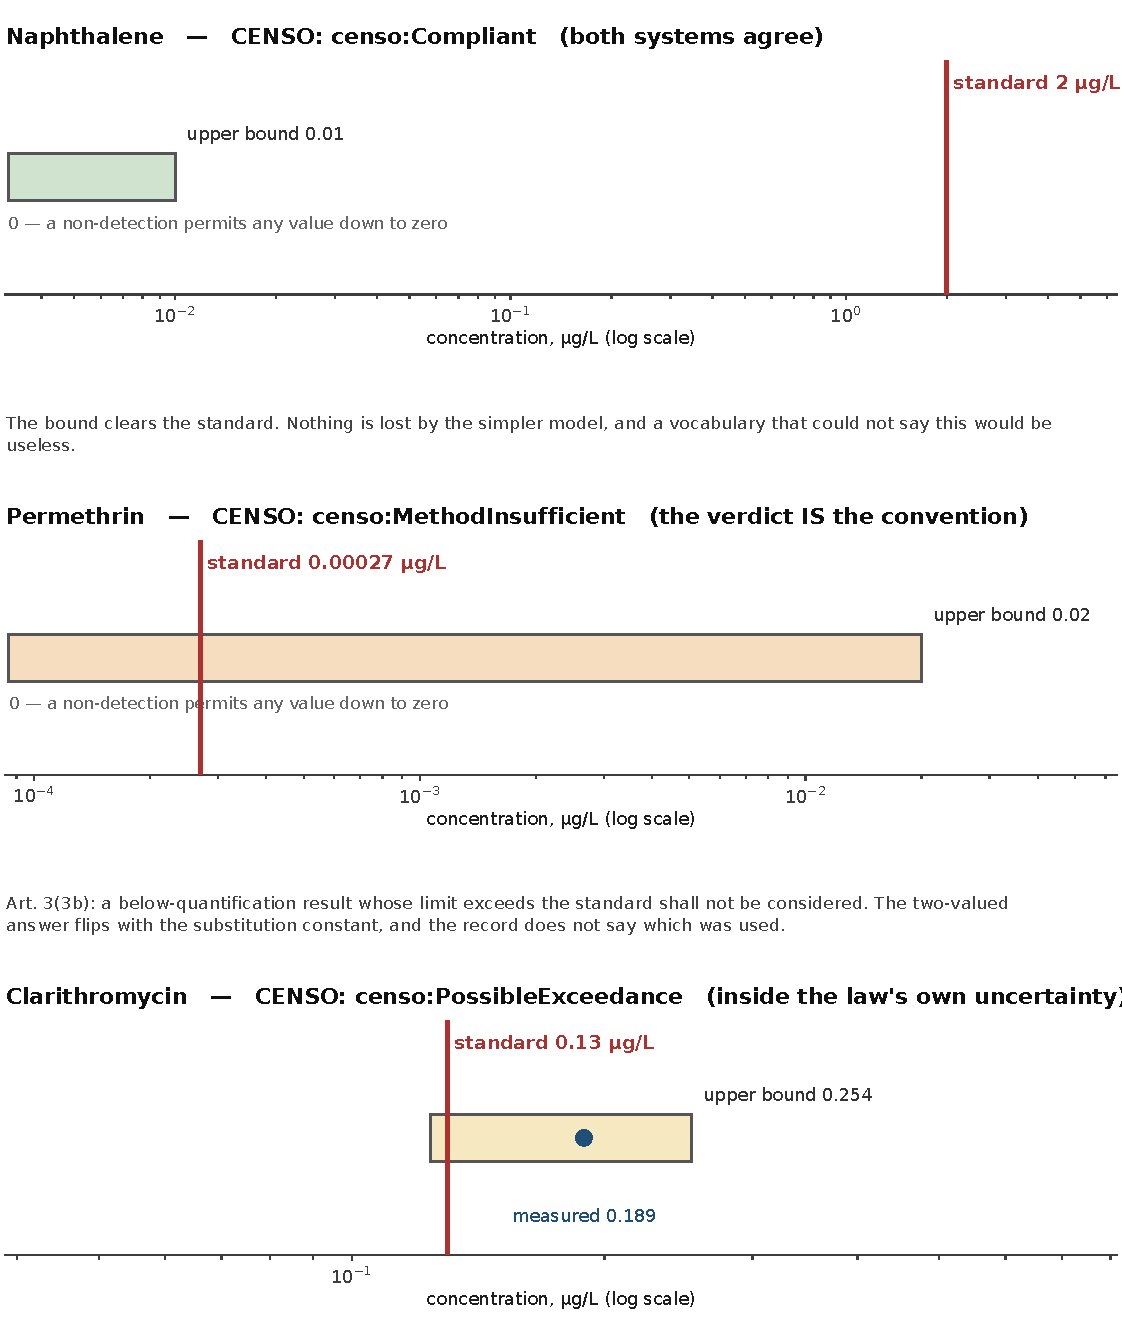
\includegraphics[width=\textwidth]{fig11_decision_walkthrough.pdf}
\caption{One real station-year per outcome class, decided by CENSO (left, the
interval the observation establishes against the standard) and by a two-valued
schema (right, at each substitution constant). The shaded bar is what the
measurement supports: for a non-detection it runs from zero, because that is
what ``not detected'' permits. Red line, the standard. Where the right-hand
column changes with the constant, the reported verdict is the convention rather
than the measurement. Every value is read from the shipped graph and ships in
\texttt{supplementary/figure\_data/fig11\_decision\_walkthrough.csv}.}
\label{fig:walkthrough}
\end{figure}

\subsection{The shipped graph is validated against the shipped shapes}
\label{sec:results-shacl}
The published shapes are run over the published graph --- \num{633960} triples
with the vocabulary loaded --- rather than over a fixture\src{scripts/18\_shacl\_validate.py}.
The shapes match \num{40000} assessed observations, \num{31167} censored ones,
\num{1159} analytical methods and \num{537} thresholds, and the run reports
\textbf{one violation type}: \num{4646} observations that cite no analytical
method. That is the unresolvable population, and it is a property of the record
rather than of the pipeline. A graph made to conform would have to invent the
datum, which is the move these shapes were corrected for once already.

Reporting a validation that does not conform requires saying which failures are
findings and which are defects, so the audit is given the list: a violation of a
declared source-data shape is recorded with its count, and any other violation
type fails the build\src{scripts/99\_audit.py}. That distinction had to be made
because until recently this stage ran for over an hour, returned
\texttt{conforms: False}, and was cited by nothing --- not the manuscript, not
the supplementary material, not the audit. The failure it was reporting was
real: the graph's concentration literals were written as bare Turtle
numerals against shapes requiring \texttt{xsd:decimal}, so
\texttt{censo:resultLowerBound 0} carried \texttt{xsd:integer} and could never match the axiom
\texttt{CensoredObservation} $\sqsubseteq$ \texttt{resultLowerBound} value
\texttt{"0.0"\^{}\^{}xsd:decimal} that the vocabulary asserts over every censored
row. No \textsc{owl} check could object, because \texttt{xsd:integer} is derived
from \texttt{xsd:decimal} and satisfies the range.

\subsection{The axioms catch real defects}
Ten test cases run against the vocabulary\src{scripts/test\_axioms.py}. Eight
inject a defect present in this dataset --- a record marked both non-detect and
quantified, a non-detection reported as an exceedance --- and all eight are
rejected, seven by OWL~2~RL entailment and one, outside the profile, by SHACL.
The other two are controls that must remain \emph{consistent}: a well-formed
graph, and one measurement carrying two verdicts under two jurisdictions'
standards. The second control matters because an earlier draft did reject it,
declaring the compliance outcomes disjoint at the class level, which would have
made Section~\ref{sec:results-dual} an inconsistency.

An OOPS!\ scan of the published distribution reports no critical pitfalls.
Three important ones were genuine and are fixed: properties lacking a domain or
range. The rest are artefacts of packaging the modules as one file for the
scanner, which leaves borrowed terms undeclared. Of the thirty-one
properties flagged as lacking an inverse, one genuinely did
(\texttt{definesThreshold}/\texttt{definedBy}) and is now declared; no inverse
was invented for the other thirty.
\section{Discussion}

\subsection{Relation to work on preprocessing sensitivity}
\label{sec:disc-lipinski}
Lipi\'nski \cite{lipinski2026sensitivity} approached the same problem from the
analysis side: on cadmium, lead and nickel, discarding below-LOQ measurements,
substituting half the LOQ and substituting the full LOQ gave substantially
different pollution patterns, and the recommendation is that studies report the
rule they used. All three yield a number; none can say the data support no
verdict at all. That is our third outcome. The comparison also needs a below-LOQ
flag and a \texttt{procedureLOQValue}; \num{25.5}\% of the record carries neither
(Section~\ref{sec:results-waterbase}), so those rows were excluded. CENSO
counts them as \texttt{UnresolvedObservation}. Metals are also the mild case:
\num{43.8}\% of Annex~I metal samples fall below the quantification limit,
against \num{77.3}\% of organic micropollutant
samples\src{scripts/22\_waterbase\_external.py}, and no comparable study covers
the newly regulated class.

\subsection{The substitution is mandated, which is the point}
\label{sec:disc-mandated}
Article~5(1) of Directive 2009/90/EC does not permit half-limit substitution, it
\emph{requires} it: a measurand below the limit of quantification ``shall be set
to half of the value of the limit of quantification
concerned''~\cite{eu2009qaqc}. Nothing in this paper is therefore a criticism of
the analysts or the authorities who do it, and the finding is not that a bad
convention is widespread. It is narrower and harder: the instrument that mandates
the substitution is the same one that sets the performance criterion the
substitution then obscures, and the record cannot show both at once. A reporter
who complies with Article~5(1) produces the \num{112034} exceedances of
Section~\ref{sec:results-wbabox} that no measurement supports, and a reporter
who does not comply produces a mean nobody can reconstruct. The way out is not a
better rule for choosing a number; it is a representation in which the bound
survives alongside whatever number the law requires to be entered, so that
Article~5(1) and Article~3(3b) can both be honoured and audited. That is what
carrying the limit onto the result buys.

\subsection{Failures that no preprocessing rule can repair}
Three findings survive any substitution rule. Where the quantification limit
exceeds the threshold, no handling of the non-detects can demonstrate
compliance: \num{17.5}\% of assessments against a European standard, and every
assessment for some pesticides (Section~\ref{sec:results-waterbase}).
Substitution only manufactures a verdict whose direction depends on the rule
chosen (Section~\ref{sec:results-wbabox}).

Several thresholds carry preconditions the record cannot satisfy: cadmium's
Annex~I standard is stated over five water-hardness classes, and the
bioavailability-corrected standards need covariates the aggregated release
lacks. A numeric threshold column carries neither the covariates nor any way to
say the standard could not be applied; CENSO returns
\texttt{PreconditionUnmet} rather than a default pass.

A threshold can also be transcribed wrongly, and nothing in a conventional
workflow would surface it. Both regulation packages released here carry a
machine-readable \texttt{transcriptionStatus}. We found the defect in our own
table: five annual averages had been parsed a factor of ten too strict, because
the extraction renders a multi-digit integer with a space between its digits,
and four maximum-allowable cells Annex~I marks ``not applicable'' had been
filled with the next number on the line. Every count against a European
standard was inflated by it. The values are now diffed against a hand-read of
the primary text on every build\src{scripts/99\_audit.py}, so a mis-parse
fails the pipeline instead of propagating --- which is the machine-readable
provenance this section argues for, applied to the argument's own inputs.

\subsection{What twelve years of reform fixed, and what it did not}
\label{sec:disc-reform}
The record shows real progress, and it should be said plainly. The share of
station-years declaring neither a censoring flag nor a limit falls from
\num{31.8}\,\% in \num{2012} to \num{0.0}\,\% in \num{2013} and has stayed there
for \num{12} years. That is not a trend, it is a step: European reporters now
record the limit in force, every time. The representational correction this paper
asks for at the point of measurement is work they have already done once.

It did not make the problem smaller. It made it \emph{visible}, which is a
different achievement, and three insufficiencies survive it.

\emph{The analytical capability did not follow the record-keeping.} Once the
limit is reported it can be tested, and the test has the same answer it had
eighteen years ago: \num{46.3}\,\% of assessments failed the \num{30}\,\%
criterion in \num{2006} and \num{47.7}\,\% in \num{2024}, with the share whose
limit exceeds the standard outright at \num{28.1}\,\% and \num{28.2}\,\%. The
limit is now always written down, and it is still too high.

\emph{The reform reached the metadata, not the value.} Censored rows carrying a
positive number stay between \num{97.2}\,\% and \num{100}\,\% across every year
the record can speak about. What was repaired is the field that says a result is
censored, not the field that still carries a substituted number in its place ---
which is why the flag is what makes the substitution reversible, and why
\num{25.5}\,\% of the historical record remains beyond repair.

\emph{The standards are moving faster than the chemistry.} Of the substances
Directive~(EU) 2026/805 adds with an annual-average standard, \num{33}\,\% place
it below \num{e-3}~\si{\micro\gram\per\litre} against \num{20}\,\% on the
legacy list --- decades in which the measured undecidable share is already
between \num{82} and \num{100}\,\%. Better reporting cannot close a gap that the
threshold is widening.

And one insufficiency is of a different kind altogether, because no analytical
improvement touches it. For cadmium, lead and nickel the standard is defined on a
quantity the reporting schema has no field for: a hardness class, or a
bioavailable concentration requiring hardness, dissolved organic carbon and pH.
That is \num{131068} assessments, \num{18.8}\,\% of every station-year a European
standard reaches (Section~\ref{sec:results-precondition}). A better laboratory
does not help here. Only a schema with somewhere to put the covariates does, and
a vocabulary that can say the standard was not applicable rather than met.

That last insufficiency is a metals problem, and it is worth saying so, because
the others are not. The censoring this paper is about is worst where the
regulation is newest: organic micropollutants are below the quantification limit
in \num{77.3}\,\% of samples against \num{43.8}\,\% for the Annex~I metals,
the substances whose limits most often exceed their own standards are
pyrethroids, neonicotinoids and pharmaceuticals rather than metals, and the
substances Directive~(EU) 2026/805 adds are almost all of that kind. Metals
supply the one failure mode that is representational rather than analytical; the
micropollutants supply the scale.

\subsection{Why the vocabularies lacked this}
SOSA/SSN was built for in-situ sensing, where a detection limit genuinely is a
property of the device and \texttt{ssn-system:DetectionLimit} is correctly a
\texttt{SystemProperty}. Trace organic monitoring analyses a transported sample
in a run with its own calibration and limits. The dominant water ontologies
inherited the sensing model, scoring heavily on sensing terminology and near
zero on sampling; CENSO puts the epistemics on the result.

That inheritance is why the shortfall is not repaired by adding a term.
Section~\ref{sec:results-separation} shows the consequence on one real record:
a limit bound to the sensor is the same fact whether the result it produced was
a measurement or a bound, so it cannot mark the difference between them, and a
vocabulary carrying it separates the two readings no better than one carrying
no limit at all. The distinction has to move with the limit, onto the result.

\subsection{Limitations}
\begin{itemize}
  \item \textbf{The standards are applied counterfactually.} Annex~I as
    consolidated in \num{2026} is applied to a record none of which was
    reported under it (Section~\ref{sec:materials}). No reporter is in breach
    of a rule that did not yet bind it and nothing here should be read as such
    a finding; what is tested is whether monitoring as performed and reported
    could decide the standards now in force --- a property of the data, not of
    the date. Section~\ref{sec:results-dual} reports how far a number moves
    when the package is changed, which is the same question asked sideways.
  \item \textbf{Anything recent rests on eight reporting authorities.} Only
    \num{8} of the \num{37} reporters contribute a post-\num{2015} river
    station-year (Section~\ref{sec:results-era}), so no claim here
    characterises \emph{current European practice}. What the coverage does
    support is narrower and is what the paper asserts: where the
    record-keeping defect was repaired, the reporter repaired it, and the
    analytical defect survived the repair.
  \item \textbf{We audit what was reported, not what was measured.} A missing
    limit may be a reporting omission rather than a laboratory one. That
    matters for blame, not for the argument: either way the record cannot
    support the verdict drawn from it.
  \item \textbf{The graph is a materialisation, not the analysis.} The
    three-valued assessment is computed for every station-year a European
    standard reaches; what is expressed as RDF is a \num{40000}-row reservoir
    sample with a fixed seed, because a pure-Python triple store cannot hold
    the full record. Nothing the paper claims rests on the sample,
    whose method-insufficient share matches the population count.
  \item \textbf{Group standards are excluded from per-substance comparison.}
    A sum standard is not a limit on any of its members, so those rows are
    reported as not individually assessable rather than assessed.
  \item \textbf{\texttt{PossibleExceedance} rests on a legal bound, not a
    reported uncertainty.} \texttt{PossibleExceedance} needs an interval around a
    quantified result. \emph{No} European release reports a per-result measurement
    uncertainty; the disaggregated release holds only
    \texttt{procedureLOQValue} and a below-quantification flag. Article~4(1) of
    Directive 2009/90/EC requires a limit of quantification at or below
    \num{30}\,\% of the standard and an expanded measurement uncertainty of
    \num{50}\,\% or below at coverage factor $k=2$, estimated at the level of
    the standard. We can count the first; WISE-6 provides nowhere to record the
    second. We therefore apply the legal maximum: the widest interval a lawful
    method could have. The construction is the ordinary decision rule of
    conformity assessment~\cite{jcgm2012conformity,eurachem2021compliance},
    in which an interval overlapping a limit yields neither acceptance nor
    rejection and ISO/IEC~17025 requires the rule to be stated~\cite{iso17025};
    what is new here is not the rule but that the outcome it produces is a
    class a query can return. It makes \texttt{PossibleExceedance} operative ---
    \num{6639} assessments --- but it is a \emph{bound}, not an estimate: none
    can be decided from what is reported, though a laboratory beating the legal
    minimum would decide some. A \emph{censored} result whose limit exceeds the
    standard has an interval straddling the threshold, so two subclasses of
    \texttt{IndeterminateCompliance} describe it; Article~3(3b) is decisive by
    the precedence of Section~\ref{sec:methods-vocab} and those assessments
    appear under \texttt{MethodInsufficient}. Both are indeterminate either way,
    so the precedence chooses the reason recorded, not the verdict.
  \item \textbf{One matrix.} River water only; lakes, transitional and coastal
    waters have their own standards and are not analysed here.
  \item \textbf{The vocabulary comparison is of published files.} An ontology
    may be used in ways its published serialisation does not show, and three
    files could not be retrieved; those are reported as unknown, not absent.
\end{itemize}

\subsection{Future work}
\label{sec:discussion-future}

\paragraph{Beyond compliance: attribution.}
The representation supports an attribution chain this paper does not pursue: a
substance's use category mapped to an expected pressure type, then compared
against the land use draining to a station. Assignments would derive from declared
substance--use--sector relations rather than from a factor interpreted after
the fact, and the chain returns ``cannot be determined'' where positive matrix
factorisation over zero-substituted data returns a number. It needs a denser
station network than any survey here provides.

\paragraph{Ontology evaluation.}
All \num{20} competency questions run against the populated graph return
non-empty answers, with their SPARQL
recorded\src{scripts/17\_run\_competency\_questions.py}. The OOPS!\ scanner
reports no critical pitfall on the distributed
ontology\src{scripts/16\_export\_for\_scanners.py}; the one it raised was a
real modelling error, now fixed. The FOOPS!\ FAIR assessment of
Section~\ref{sec:methods-repro} leaves two kinds of work outstanding. Three
missing annotations --- a citation, a publisher, an issue date --- are edits to
the file and will land with the archived release, since two of them are not
determinable until it has a DOI. The other three are absence from a public
registry, which is a submission rather than an edit and which we have not made:
a vocabulary should be indexed where people look for one, and until it is, the
reuse this paper argues for costs a reader more than it should.

\paragraph{The taxonomy is declared but not yet interrogated.}
The four subclasses of \texttt{IndeterminateCompliance} are materialised and
counted (Section~\ref{sec:results-wbabox}), and no competency question asks the
graph to group an indeterminate verdict by its reason. That query is the direct
test of whether the subtyping earns its place, and it is the first addition the
question set should take.

\subsection{Implications}
For monitoring programmes the recommendation costs nothing at the point of
measurement: record with every result the limits of the run that produced it ---
the quantification limit the two provisions are written about, and the detection
limit where the method states one. That alone decides whether censoring can be
reconstructed.

For regulators, an environmental quality standard below the achievable limit of
quantification is unenforceable, and the mismatch is discoverable automatically
once both are machine-readable.

For the semantic web community, a standard's implicit measurement modality
propagates into every extension built on it: until SOSA's sampling vocabulary
is connected to analytical provenance, sample-and-analyse domains will keep
reaching for a sensor model that does not fit.

\section{Conclusions}

A non-detection is an upper bound and an open-world statement. Recording it as a
zero replaces that statement with a number; routine data models offer nowhere
else to put it.

Across \num{4190833} river station-years, \num{44.9}\% of samples lie below the
quantification limit, and \num{25.5}\% of station-years carry neither a censoring
flag nor a limit, so a zero and a measured trace cannot be told apart. Where a
standard exists, \num{40.1}\% of assessments come from a method failing the
performance criterion of Directive 2009/90/EC, and \num{17.5}\% from one whose
limit exceeds the standard outright --- results Article~3(3b) requires to be set
aside and a two-valued pipeline records as compliance.

The record is not one era. The share declaring neither a flag nor a limit falls
from \num{49.7}\% before \num{2015} to \num{0.0}\% after, and the \num{8}
authorities reporting in both periods account for all of it. The
representational correction is work these reporters have already done, under an
unchanged standard. The analytical failure does not move: on \num{2024} alone,
with every limit reported, \num{47.7}\,\% of assessments still come from a
method that cannot decide its own standard.

Over \num{696168} assessments --- station-years, not samples --- the same
records yield a \num{3.4}-fold range in exceedances according to whether a
non-detection is entered at zero, half the limit or the limit; \num{14505}
are exceedances the law can affirm: the number a two-valued pipeline reports is
fixed by the convention, not by the chemistry. Annex~I also
states a second standard on a different unit of observation, and reading the
\num{96597294} individual samples of the disaggregated release leaves
\num{9.7}\,\% of them undecidable for the same reason, with \num{25.6}\,\% of
the station-years assessable under both standards receiving different verdicts
--- two answers a single threshold column cannot hold at once.

A two-valued model cannot express these states. CENSO can: it binds the
quantification limit to the result it bounds, and makes \emph{cannot be
determined} the third of the three outcomes the Directive admits --- subtyped by
the reason, so that an unmeasurable standard, an unreported bound, an
inapplicable one and an interval straddling the limit are four answers and not
one shrug. Its axioms reject all eight defects drawn
from this dataset and accept both controls, and expressing the record in it
loses nothing: every row classified in the graph lands where the streaming
count puts it. Applying two jurisdictions to
the same observations changes \num{17.7}\% of the outcomes both regulate, with
no code change. Of the \num{21} ontologies parsed, none combines these
capabilities and none carries a censoring status at all, and the shortfall is
not lexical: on one real record \num{20} of them cannot separate a non-detection
from a measurement reporting the same number,
because the two readings translate to the same facts in each. CENSO makes them
incompatible rather than merely differently labelled.

The corrective for practice is cheap: record the quantification limit with every
result, per analytical method. The corrective for representation is to stop
treating ``not detected'' as a number.

\section*{Declaration of competing interest}
The authors declare no competing financial interests or personal relationships
that could have appeared to influence the work reported in this paper.

\section*{CRediT authorship contribution statement}
% DRAFT --- every role below must be confirmed by the named author before
% submission. Misattributing a CRediT role is a research-integrity matter, not
% a formatting one.
\textbf{Recep Can Altınbağ:} Conceptualization, Methodology, Software,
Formal analysis, Data curation, Validation, Visualization, Writing --- original
draft. \textbf{Mehmet Tahir Sandıkkaya:} Methodology, Supervision,
Writing --- review \& editing. \textbf{Ulaş Pekyavaş:} Investigation,
Writing --- review \& editing.

\section*{Declaration of generative AI and AI-assisted technologies
in the writing process}
% Elsevier requires this statement when a generative tool assisted the WRITING.
% Fill in the tool and the purpose truthfully; the authors remain responsible
% for every claim regardless of what assisted its drafting.
During the preparation of this work the authors used
\pending{tool and purpose}. After using this tool the authors reviewed and
edited the content as needed and take full responsibility for the content of
the publication.

No figure in this article was generated or altered by a generative model. Every
figure is drawn by \texttt{scripts/90\_figures.py} from the tabular data
deposited with the article, the values behind each mark are shipped in
\texttt{figure\_data/}, and any reader can regenerate the figures from the
public source data without contacting the authors.

\section*{Data availability}
The ontology, both regulation packages, the processing pipeline, every SPARQL
query and all evaluation outputs are openly available (see Software
availability). The measurements are the EEA's Waterbase --- Water Quality ICM,
aggregated release, downloadable at
\url{https://www.eea.europa.eu/en/datahub/datahubitem-view/fbf3717c-cd7b-4785-933a-d0cf510542e1};
no application or permission is required, so every number here can be
re-derived independently. Three files from that item are used, and the scripts
name them: \texttt{WISE6\_AggregatedData} for the annual means every
headline number rests on, \texttt{WISE6\_SpatialObjects\_DerivedData} for the
station coordinates in Figure~\ref{fig:europe-map}, and
\texttt{WISE6\_DisaggregatedData} for the individual samples the
maximum-allowable standard is defined against (Section~\ref{sec:results-mac}).
The last is distributed in a Deflate64 archive that Python's \texttt{zipfile}
cannot open; the pipeline falls back to \texttt{7z} or \texttt{bsdtar}, and
skips that stage with a message rather than failing if the file is absent.

\bibliographystyle{elsarticle-harv}
\bibliography{refs}

\end{document}
